\documentclass[a4paper,12pt,oneside]{report}%FinalView
%\documentclass[draft,a4paper,12pt,oneside]{report}%draftView

\usepackage{indentfirst}

%Page Geometry
\usepackage[
	top=3cm,
	bottom=2cm,
	left=2cm,
	right=2cm,
	%bindingoffset=2cm, %Adds a Binding offset for printed documents
	marginparwidth=6cm, %Adds Overflow Width to Rigth Margin 
	marginparsep=3mm %Gap between right margin and right overflow margin
	]{geometry}
%\usepackage{showframe} % UNCOMMENT TO SHOW BORDERS REPRESENTING YOUR PAGE ARANGMENT
%\usepackage[cam,center,a3]{crop}%Extends PageView

\usepackage[T1]{fontenc}
\usepackage[none]{hyphenat} %Prevents hyphen words
\usepackage{soul}%alows highlighting with \hl{}
\usepackage{setspace}
%\doublespace
\onehalfspacing

\usepackage{graphicx}
\graphicspath{{./images/}}
\usepackage[center]{caption}
\usepackage{subcaption}
\usepackage{placeins}
\usepackage{float}
%\captionsetup[sub]{labelsep=newline}
%\usepackage{subfigure}

\usepackage[colorinlistoftodos]{todonotes} %Adds todonotes to margin
\usepackage{marginnote} %Adds basic margin notes 	\marginpar{This is a sample margin note....}
\sloppy %prevents margin overflow
\usepackage[hyperfigures=true,colorlinks=true,linkcolor=black]{hyperref}%hyperlinks
\usepackage[toc]{glossaries}%glossary
\makeglossaries%create glossary
\usepackage{tikz}
\usetikzlibrary{patterns}
\usepackage{pgfplots}
\usepackage{color}
\usepackage{hyperref}
\hypersetup{urlcolor=blue,linkcolor=black,citecolor=black,colorlinks=true}
\usepackage{array,multirow}
\usepackage[numbers,sort&compress]{natbib}
\usetikzlibrary{plotmarks}
\usepackage{amsmath}
\usepackage{mathpazo}
%\usepackage{fancyhdr}
%\pagestyle{fancy}
\usepackage{numprint}
\usepackage{sistyle}
\usepackage{booktabs}
%\DeclareMathOperator\erfc{erfc}
%\DeclareMathOperator\erf{erf}
%\DeclareMathOperator\F{F}
%\DeclareMathOperator\G{G}
\usepackage{lscape}
\setlength{\unitlength}{1cm}
\usepackage{amssymb} 
\usepackage[parfill]{parskip}
\usepackage[nottoc,numbib]{tocbibind}
\usepackage{rotating, graphicx}
\usepackage{pdflscape}
\usepackage[toc,page]{appendix}
\pgfplotsset{minor grid style={dashed,gray!50}}
\pgfplotsset{major grid style={black}}
\usepackage{threeparttable}
\usepackage[version=2]{mhchem}
\usepackage{array}
\newcolumntype{L}[1]{>{\raggedright\let\newline\\\arraybackslash\hspace{0pt}}m{#1}}
\newcolumntype{C}[1]{>{\centering\let\newline\\\arraybackslash\hspace{0pt}}m{#1}}
\newcolumntype{R}[1]{>{\raggedleft\let\newline\\\arraybackslash\hspace{0pt}}m{#1}}
\setcounter{tocdepth}{4} %Adds subsubsection numbers
\setcounter{secnumdepth}{4} %Adds subsubsections to ToC
\usepackage{verbatim} %Allows multiple line comments
\usepackage{titletoc}
\usepackage{textcomp} %copywrite symbol

%Allow costume names for sections like Bibiography
\renewcommand\bibname{BIBLIOGRAPHY}
\renewcommand{\contentsname}{TABLE OF CONTENTS}
\renewcommand{\listfigurename}{LIST OF FIGURES}
\renewcommand{\listtablename}{LIST OF TABLES}
\renewcommand{\glossaryname}{GLOSSARY}

%My Commands
\newcommand{\MgZnCa}{Mg$_{65}$Zn$_{30}$Ca$_{5}$}
\newcommand{\ZrCuNiAl}{Zr$_{55}$Cu$_{30}$Ni$_{5}$Al$_{10}$}
\newcommand{\ZrCuAl}{Zr$_{65}$Cu$_{27.5}$Al$_{7.5}$}
\newcommand{\Tg}{$T_{g}$}
\newcommand{\Tx}{$T_{x}$}
\newcommand{\Tm}{$T_{m}$}
\newcommand{\Tl}{$T_{l}$}
\newcommand{\TgTm}{$T_{g}/T_{m}$}
\newcommand{\TgTl}{$T_{g}/T_{l}$}
\newcommand{\n}{$\eta$}
\newcommand{\Rc}{$R_{c}$}
\newcommand{\dTg}{$\delta T_{g}$}
\newcommand{\Tsub}{$T_{sub}$}
\newcommand{\Tf}{$T_{f}$}
\newcommand{\Tk}{$T_{k}$}
\newcommand{\Tonset}{$T_{onset}$}
\newcommand{\degree}{$^{\circ}$}
\newcommand{\Cp}{$C_{p}$}
\newcommand{\p}{$\rho$}


%Glossary
\newacronym{fda}{FDA}{Food and Drug Administration}
\newacronym{tga}{TGA}{Therapeutic Goods Administration}
\newacronym{unsw}{UNSW}{University of New South Wales}

\newacronym[longplural={metallic glasses}]{mg}{MG}{metallic glass}
\newacronym[longplural={bulk metallic glasses}]{bmg}{BMG}{bulk metallic glass}
\newacronym[longplural={glass forming abilities}]{gfa}{GFA}{glass forming ability}
\newacronym[longplural={ultrastable metallic glasses}]{smg}{SMG}{ultrastable metallic glass}
\newacronym[longplural={thin film metallic glasses}]{tfmg}{TFMG}{thin film metallic glass}
\newacronym[longplural={ultrastable glasses}]{usg}{USG}{ultrastable glass}
\newacronym{stz}{STZ}{shear transfer zone}
\newacronym{sro}{SRO}{short range order}
\newacronym{mro}{MRO}{medium range order}
\newacronym{lro}{LRO}{long range order}
\newacronym{Rc}{$R_{c}$}{critical cooling rate} %K/s
\newacronym{scl}{SCL}{super cooled liquid}
\newacronym{sclr}{SCLR}{super cooled liquid region}
\newacronym[longplural={fragilities}]{m}{$m$}{fragility}
\newacronym{ttt}{TTT}{time-temperature-transformation}
\newacronym{cct}{CCT}{continuous cooling transformation}
\newacronym{vft}{VFT}{Vogel--Fulcher--Tammann}

\newacronym{E}{E}{young's modulus} %GPa
\newacronym{n}{$\eta$}{viscosity} %Pa S   NOTE overpotential is nOver
\newacronym{p}{$\rho$}{density} %kg/m^3
\newacronym{V}{$V$}{volume} %m^3
\newacronym{v}{$v$}{specific volume} %m^3/kg
\newacronym{Vm}{$V_{m}$}{molar volume} %m^3/mol
\newacronym{G}{$G$}{Gibb's Free Energy} %J
\newacronym{G*}{$\Delta G^*$}{nucleation barrier energy} %J
\newacronym{ysl}{$\gamma_{SL}$}{surface energy} %J/m^2
\newacronym{dG}{$\Delta G$}{change in Gibb's Free Energy} %J
\newacronym{dGV}{$\Delta G_{V}$}{reduction in volume energy} %J/m^3
\newacronym[longplural={nucleus radii}]{r}{$r$}{nucleus radius} %m
\newacronym[longplural={critical radii}]{r*}{$r^{*}$}{critical radius} %m
\newacronym{M}{$M$}{indentation modulus}

\newacronym{Cp}{$C_{p}$}{heat capacity} %J
\newacronym{cp}{$c_{p}$}{specific heat capacity} %J / gK
\newacronym{H}{$H$}{enthalpy} %J
\newacronym{h}{$h$}{specific enthalpy} %J / g
\newacronym{H0}{$H_{0}$}{absolute zero enthalpy} %J
\newacronym{S}{$S$}{entropy} %J/K
\newacronym{s}{$s$}{specific entropy} %J/gK

\newacronym{dc}{DC}{direct current} %I
\newacronym{Vp}{$V$}{potential} %V
\newacronym{Ea}{$E_{A}$}{applied potential} %V
\newacronym{Eocp}{$E_{OCP}$}{open circuit potential} %V
\newacronym{Ecorr}{$E_{corr}$}{corrosion potential} %V
\newacronym{i}{$i$}{current density} %A/cm^2
\newacronym{i0}{$i_{0}$}{exchange current density} %A/cm^2
\newacronym{icorr}{$i_{corr}$}{corrosion current density} %A/cm^2
\newacronym{nOver}{$\eta$}{overpotential} %V
\newacronym{ocp}{OCP}{open circuit potential}

\newacronym{re}{RE}{rare earth element}
\newacronym{pcl}{PCL}{polycaprolactone}
\newacronym{tmax}{$t_{max}$}{maximum sample thickness} %mm
\newacronym{B}{$\beta$}{Tafel slope}
\newacronym{ok}{$\theta _{k}$}{proportion along the energy landscape}

\newacronym{T}{$T$}{temperature} %K
\newacronym{Tf}{$T_{f}$}{fictive temperature} %K
\newacronym{Tg}{$T_{g}$}{glass transition temperature} %K
\newacronym{Tg0}{$T_{g0}$}{normallised glass transition temperature} %K
\newacronym{Ti}{$T_{i}$}{intersection temperature} %K
\newacronym{Tk}{$T_{k}$}{Kauzmann temperature} %K
\newacronym{Tl}{$T_{l}$}{liquidus temperature} %K
\newacronym{Tm}{$T_{m}$}{melting temperature} %K
\newacronym{Tonset}{$T_{onset}$}{onset temperature} %K
\newacronym{Trg}{$T_{rg}$}{reduced glass transition temperature} %Tg/Tm
\newacronym{Tsub}{$T_{sub}$}{substrate temperature} %K
\newacronym{Tx}{$T_{x}$}{crystallisation temperature} %K
\newacronym{dT}{$\Delta T$}{super cooled liquid region} %K
\newacronym{dTg}{$\delta T_{g}$}{enhanced glass transition temperature} %K
\newacronym{ht}{$\beta$}{heating rate} %K/min

\newacronym{vd}{VD}{vapour deposition}
\newacronym{cvd}{CVD}{chemical vapour deposition}
\newacronym{pvd}{PVD}{physical vapour deposition}
\newacronym{pld}{PLD}{pulse laser deposition}
\newacronym{uhv}{UHV}{ultrahigh vacuum}
\newacronym{tpf}{TPF}{thermoplastic forming}
\newacronym{sccm}{SCCM}{standard cubic centimetres per minute}

\newacronym{abed}{ABED}{angstrom beam electron diffraction}
\newacronym{afm}{AFM}{atomic force microscopy}
\newacronym{dsc}{DSC}{differential scanning calorimetry}
\newacronym{dta}{DTA}{differential thermal analysis}
\newacronym{eds}{EDS}{energy-dispersive X-ray spectroscopy}
\newacronym{epma}{EPMA}{electron probe microanalyzer}
\newacronym{icp}{ICP}{inductively coupled plasma mass spectrometry}
\newacronym{fib}{FIB}{focused ion beam}
\newacronym{sem}{SEM}{scanning electron microscopy}
\newacronym{stem}{STEM}{scanning transmission electron microscopy}
\newacronym{tem}{TEM}{transmission electron microscopy}
\newacronym{hrtem}{HRTEM}{high-resolution transmission electron microscopy}
\newacronym{xrd}{XRD}{X-ray diffraction}
\newacronym{xrr}{XRR}{X-ray reflectivity}
\newacronym{pdp}{PDP}{potentiodynamic polarisation}
\newacronym{pdf}{PDF}{pair distribution function}

\newacronym{rt}{RT}{room temperature}
\newacronym{comp}{CP}{commercially pure}
\newacronym{tpi}{TPI}{teeth per inch}
\newacronym{rpm}{RPM}{rotations per minute}
\newacronym{mdl}{MDL}{method dection limit}
%Inputs Preamble for its .tex
\usepackage[color]{showkeys}%Shows cross ref paths

\begin{document}

%%%%%%%%%%%%%%%%%%%%%%%%%%%%%%%%%%%%%%%%%%%%%%%%%%%%%%%%%%%%%%%%%%%%%%%%%%

%Table of Contents
%\clearpage
\newpage
\tableofcontents\newpage
\addcontentsline{toc}{chapter}{TABLE OF CONTENTS}
\listoffigures\newpage
\listoftables\newpage
%\clearpage %% start of main matter

%%%%%%%%%%%%%%%%%%%%%%%%%%%%%%%%%%%%%%%%%%%%%%%%%%%%%%%%%%%%%%%%%%%%%%%%%%

\chapter{EXPERIMENTAL PROCEDURE}
\glsresetall

\section{Semi-Crystalline Target Manufacture} 

\subsection{Base Elements}

\subsection{Induction Furnace Melting}
\subsubsection{Induction Furnace Equipment}

\subsubsection{Crucibles}

\subsubsection{Melt Cycle}

\subsubsection{Gravity Casting}

\subsection{Final Shaping}

\subsubsection{Riser Removal} 

\subsubsection{Target Extraction}

\subsubsection{Target Rounding}

\subsubsection{Target Polishing}

\section{Crystalline Target Manufacture}

\subsection{Induction Furnace Melting}

\subsubsection{Melt Cycle}

\subsubsection{Gravity Casting}

\subsection{Final Shaping}

\subsubsection{Sectioning of Targets}

\subsubsection{Target Rounding}

\subsubsection{Target Polishing}

\section{DC Magnetron Sputtering}

\subsection{DC Magnetron Sputtering Equipment}

\subsection{Depostion of Thin Films}

\subsection{Target Lifespan}

\section{Examined Substrates} 

\subsection{Silicon Wafer Substrate}

\subsection{Water Soluble Substrate} 

\subsection{BMG Substrate}

\subsection{Polycaprolactone (PCL) Scaffolds}

\section{Thin Film Characterisation}

\subsection{Physical and Chemical Properties}

\subsection{Quality of Deposition} 

\subsection{Biocompatibility and Bioabsorption} 

\subsection{Master alloy}

\subsection{\acrshort{dc} magnetron sputtering}
 
\subsection{Stylus profiler analysis}

\subsection{\acrshort{eds} analysis}

\subsection{\acrshort{dsc} characterization}

\subsection{\acrshort{xrd} characterization}


%%%%%%%%%%%%%%%%%%%%%%%%%%%%%%%%%%%%%%%%%%%%%%%%%%%%%%%%%%%%%%%%%%%%%%%%%%

\chapter{EXPERIMENTAL PROCEDURE}
\glsresetall

\section{Semi-Crystalline Target Manufacture} \label{sec:TargetManufacture}
The production of thin films by \gls{pvd} requires targets of appropriate composition for the desired film stoichiometry. These master alloy targets were produced by induction melting of pure constituent element ingots.

\subsection{Base Elements}
The \MgZnCa~ master alloy were prepared from pure constituent element ingots of Mg (99.85 wt\%), Zn (99.995 wt\%), and Ca (99.8 wt\%). Each element ingot was polished and filed to removal surface contamination and oxides. The ingots were cut to size on either a Struers Labotom-3 or a Struers Discotom-6 auto-cutter at a feed rate of no more than $0.2~ mm/s$ at $2850 - 3420$ \acrshort{rpm} (Figures \ref{fig:AutoCutter} and \ref{fig:MgIngot}).

%code to put 2 images side by side in a figure
\begin{figure}[htbp]
	\centering
	%Image 1
	\begin{subfigure}[htbp]{0.49\textwidth}
		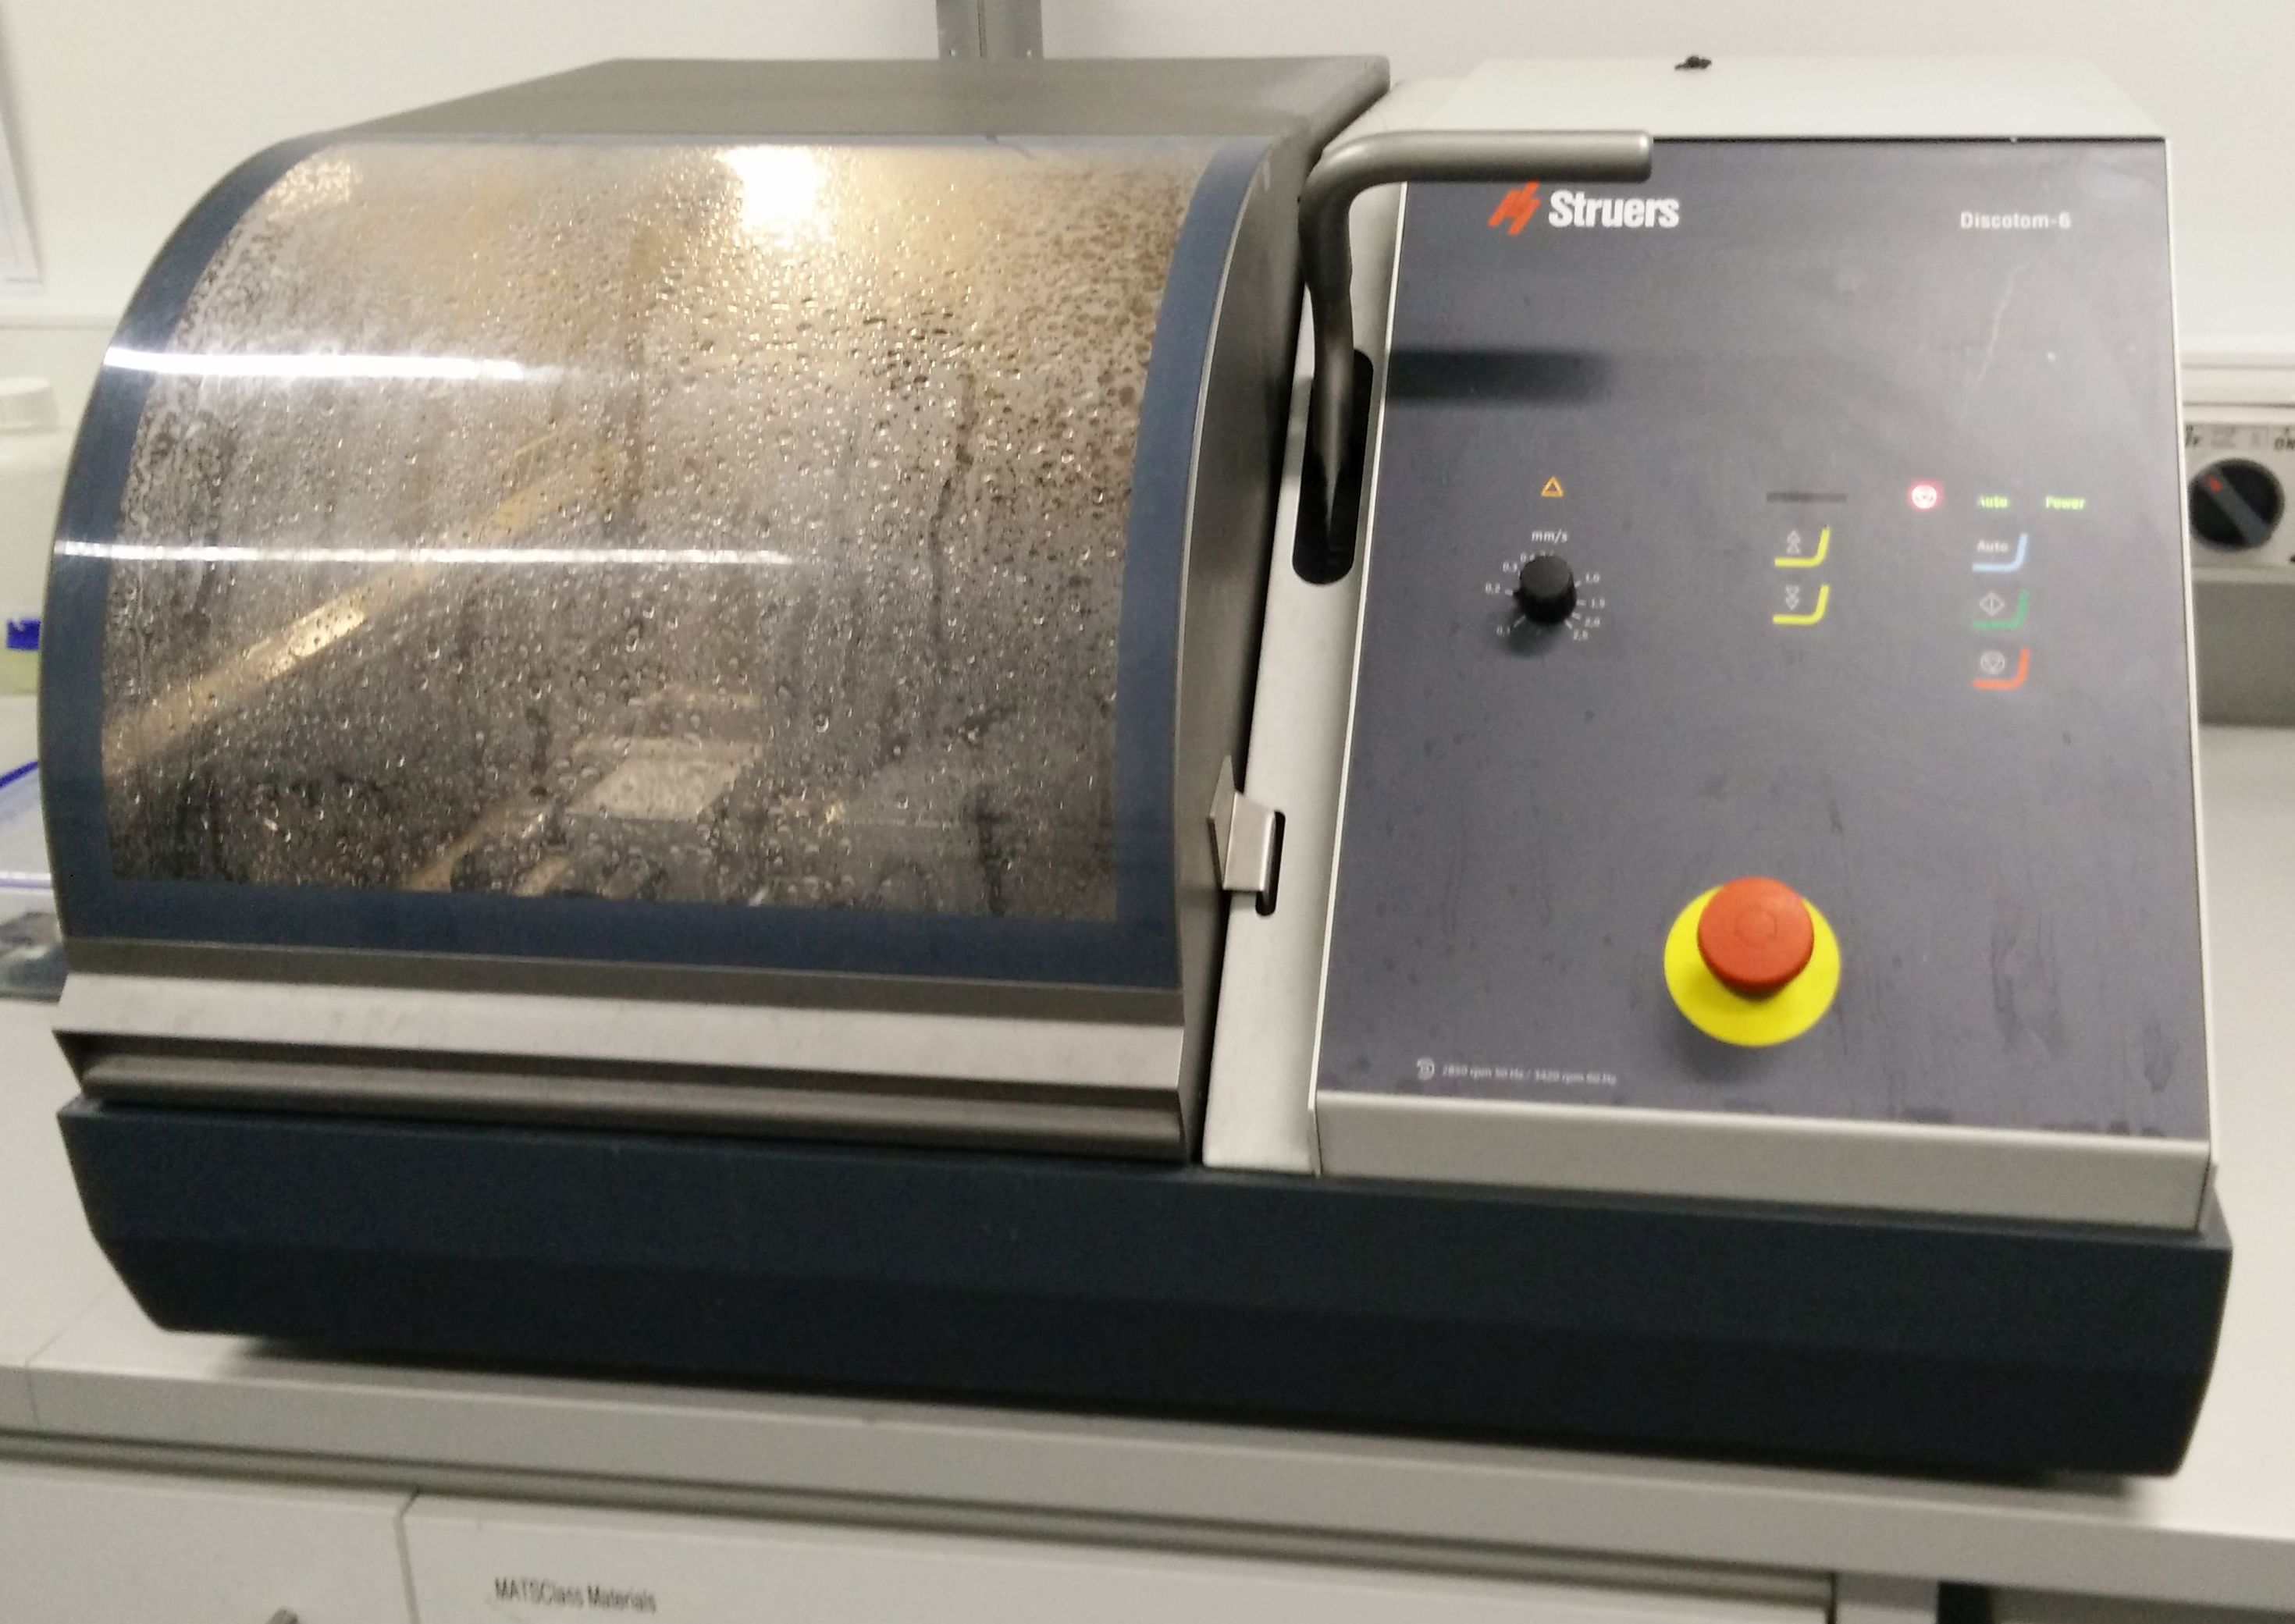
\includegraphics[width=\textwidth]{Ex_AutoCutter.jpg}
		\caption{}
		\label{fig:AutoCutter}
	\end{subfigure}
	%Image 2
	\begin{subfigure}[htbp]{0.30\textwidth}
		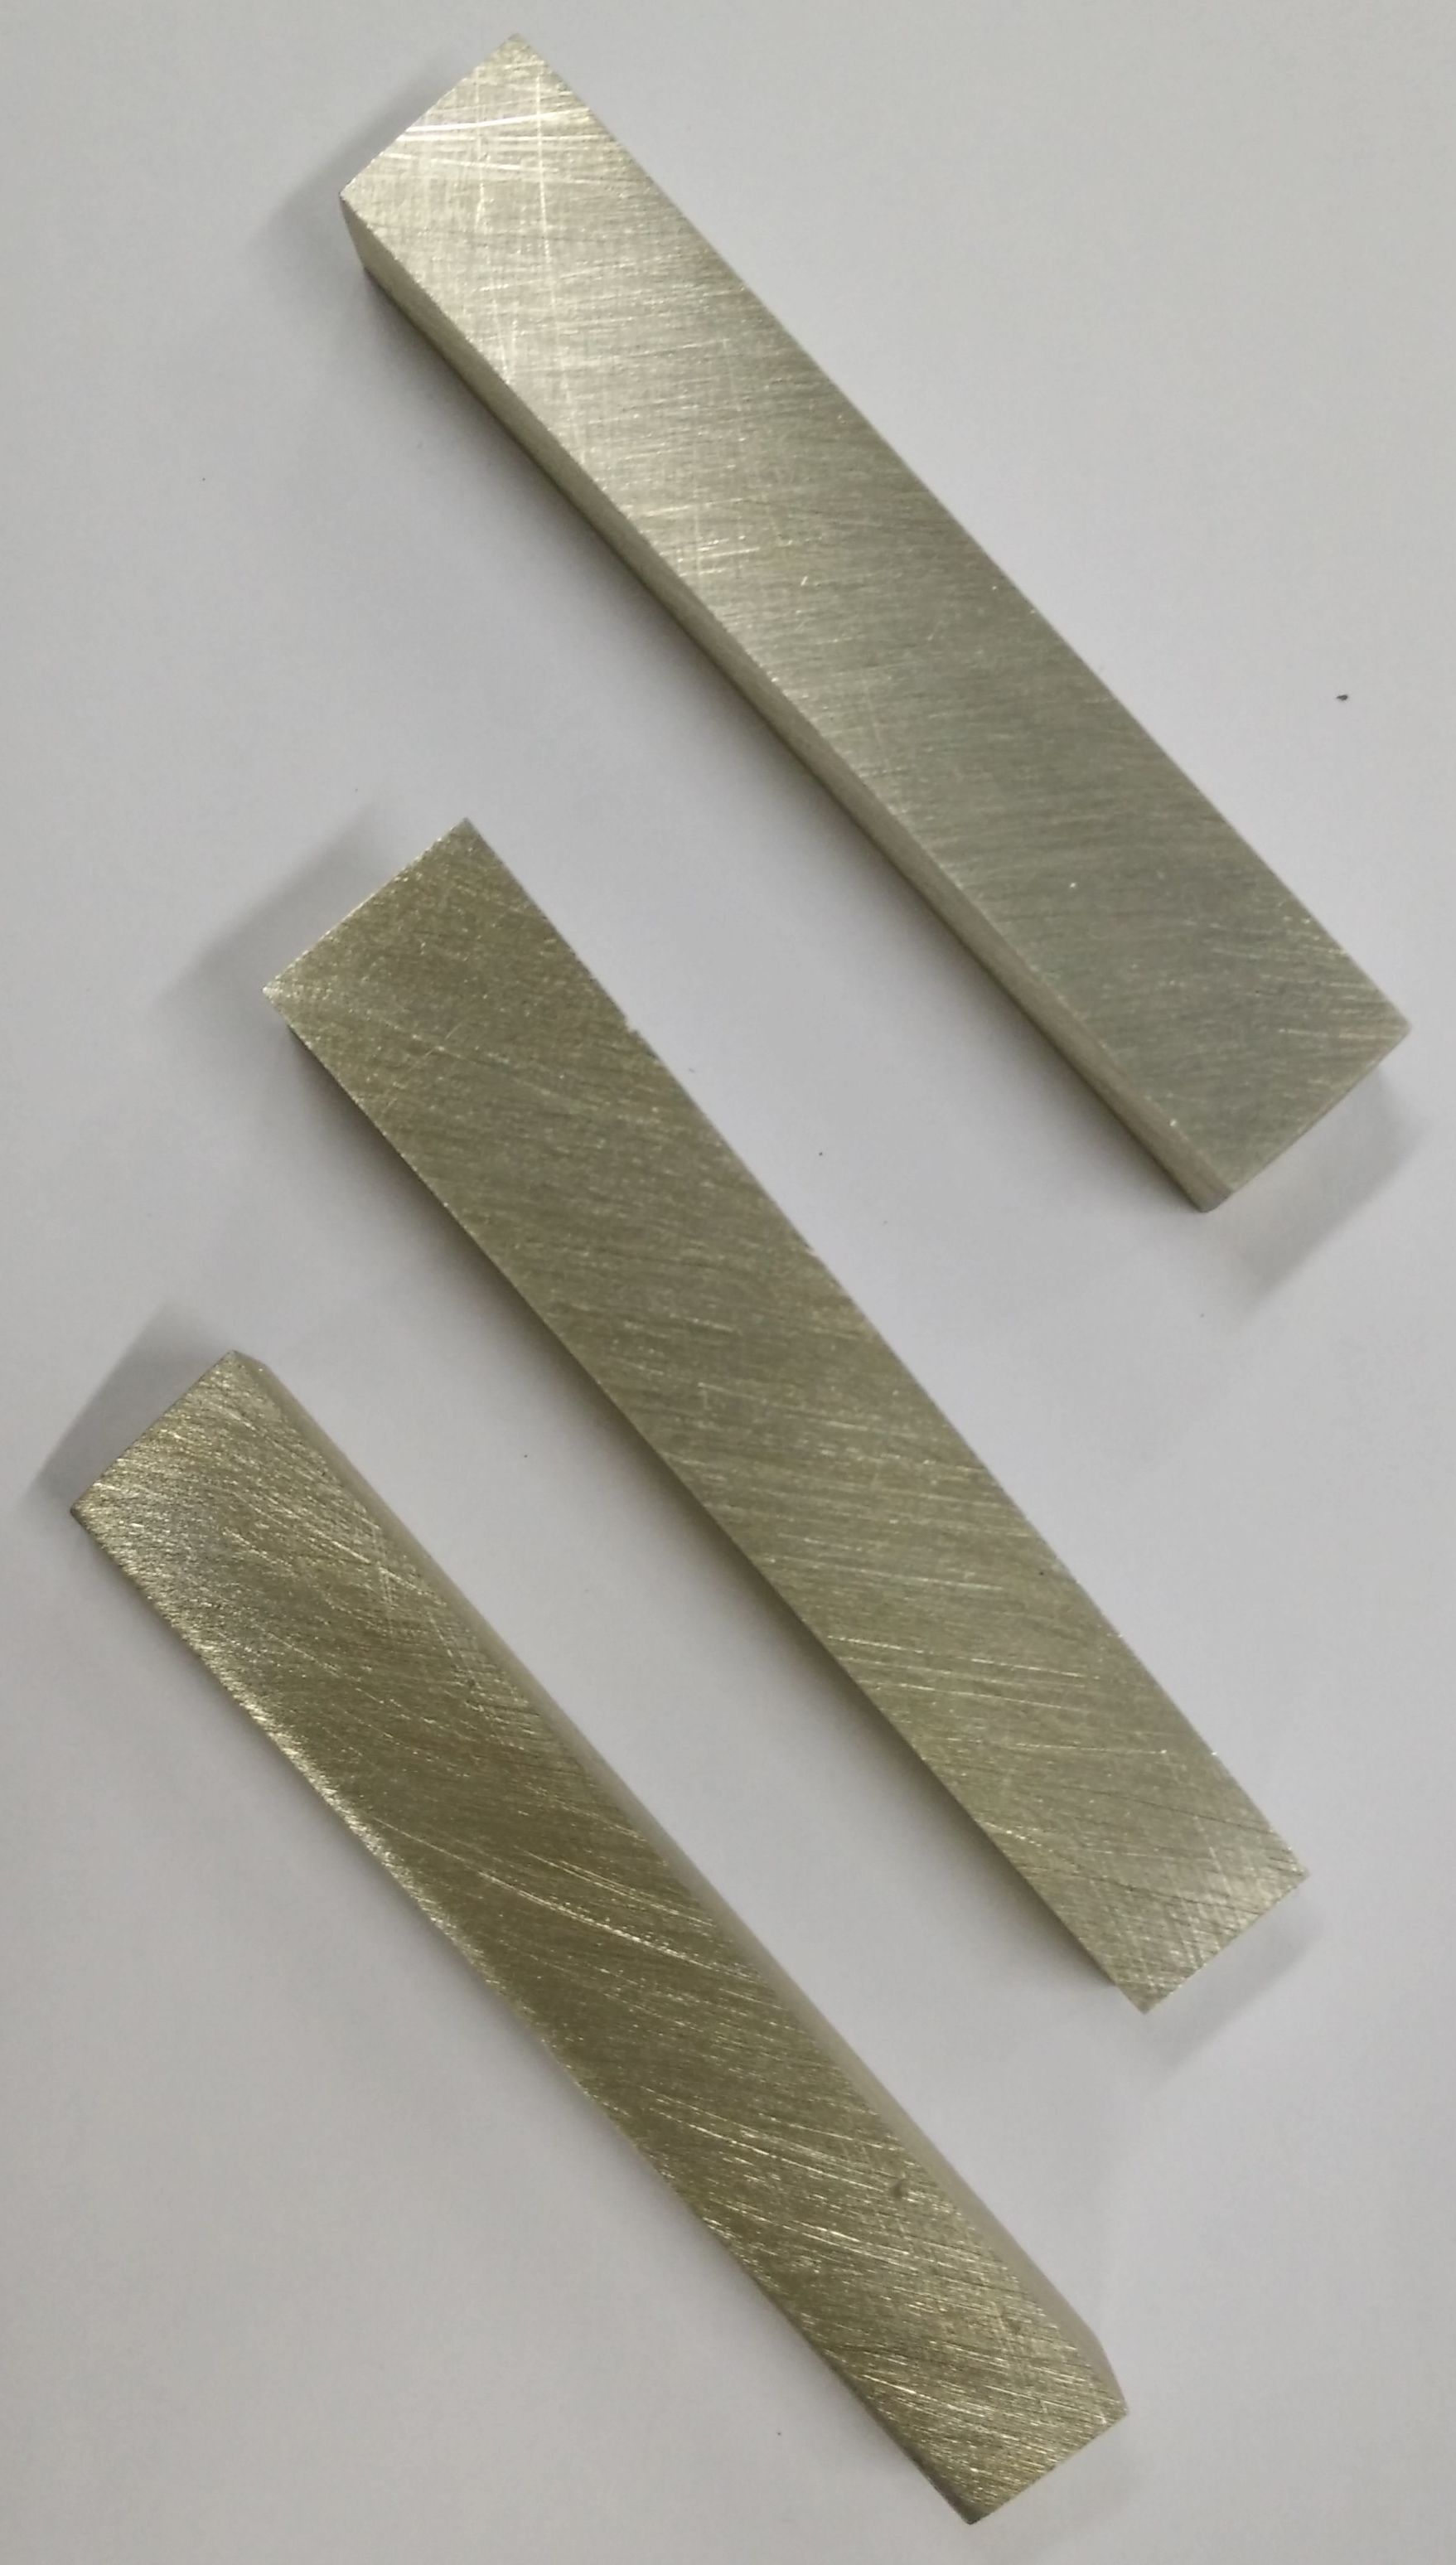
\includegraphics[width=\textwidth]{Ex_Mg_Cut_Ingot.jpg}
		\caption{}
		\label{fig:MgIngot}
	\end{subfigure}
	\caption{(a) Struers Discotom-6 auto-cutter. (b) Cut and fully deoxided Mg ingot ready for casting.}%global caption
	\label{fig:Cutter_MgIngot}
\end{figure}

The total weight of each constituent element required for a master alloy charged was automatically calculated by a developed MS Excel workbook, Figure \ref{fig:ChargeSheet}. This tool auto-computes the required weights of each element from the prepared ingot innovatory, checks the expected master alloy composition, and provides a space for notes on the entire process (i.e. heating cycles, observations, possible future refinements, etc.).

%single image
\begin{figure}[htbp]
	\centering
	\includegraphics[width=0.99\textwidth]{Ex_ChargeSheet.png}
	\caption{Screenshot of the MS Excel workbook developed for auto-calculating master alloy charge weights, checking expected master alloy composition, and taking notes for future refinements.}
	\label{fig:ChargeSheet}
\end{figure}

\subsection{Induction Furnace Melting}
\subsubsection{Induction Furnace Equipment}
The \MgZnCa~ master alloy was prepared from the base element ingots by an in house induction furnace and casting facility (Figures \ref{fig:CastingSchematic} and \ref{fig:LawsCasting}). The facility has a maximum temperature of 1300\degree C, heating rate of 500\degree C/min, and vacuum and dynamic gas melting capability \cite{Laws2007}. The dyanmic gas flow rate can be varied from $0-200~ cm^{3}/min$, and temperature regulated by a K-type thermocouple \cite{Laws2007}. The casting capabilities allow for conventional gravity casting, inverted injection casting, vacuum/suction casting or combination injection/vacuum casting \cite{Laws2007}.

%single image
\begin{figure}[htbp]
	\centering
	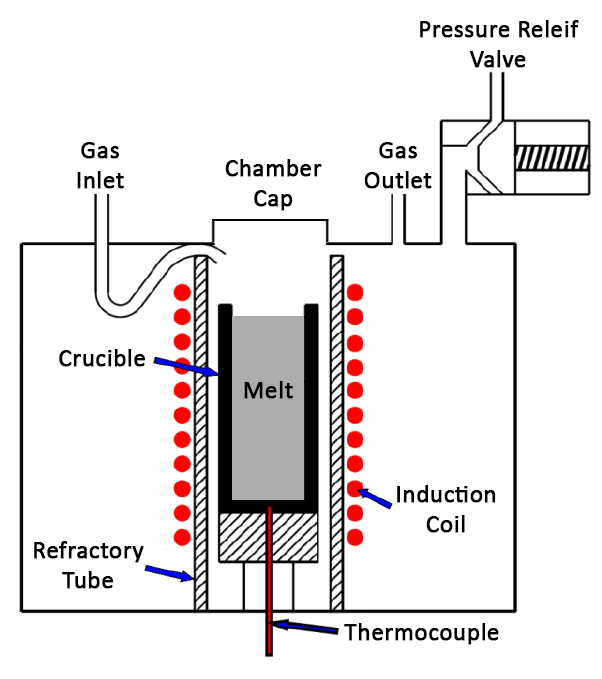
\includegraphics[width=0.75\textwidth]{Ex_Laws_Induction_Schematic.png}
	\caption[Schematic of induction casting melting chamber.]{Schematic of induction casting melting chamber. Adapted from \cite{Laws2007}.}
	\label{fig:CastingSchematic}
\end{figure}

\subsubsection{Crucibles}
Boron nitride coated graphite crucibles were used for the melting because the coating is inert with molten Mg. Two sizes are available for the facility, $32~ mm$ and $34~ mm$ diameter, by $85~ mm$ in length, allowing for maximum usable charge volumes of $40$ and $60~ cc$ respectively. The Mg and Zn ingots were placed in the bottom of the crucible with maximum wall contact, with the Ca being added on the top, Figure \ref{fig:CrucibleCharge}.

\subsubsection{Melt Cycle}
The prepared crucible was sealed in the induction furnace chamber, evacuated and purged with Ar (99.997 vol.\% purity) five times before starting a continues circulating Ar flow through the chamber to prevent oxidation of the melt (Figure \ref{fig:CastingSchematic}). The crucible charge was induction melted at 700\degree C for a couple minutes and stirred with a tungsten rod. The melt was then partially solidification at 385\degree C, remelted and stirred at 650\degree C, partially re-solidification at 385\degree C, and remelted and stirred again at 650\degree C. The melt was then cooled to a casting temperature of $500- 510$\degree C and removed from the melt chamber by the incorporated raising bar. This heating/cooling cycle between the alloy's solidus/liquidus region and the liquid state helps ensure a homogeneous alloy melt. 

\subsubsection{Gravity Casting}
For naturally cooled gravity casting the melt was manually poured into a prepared copper plate mould. The casting cavity is $100~ x~ 50~ mm$ with spacers allowing for thicknesses ranging from $2~ mm$ to several $mm$, with $4~ mm$ plate proving the most practical (Figures \ref{fig:LawsMould} and \ref{fig:FilledMould}). The $4~ mm$ plate variation has a volume of approximately $20~ cc$ with the riser holding an additional $15.5~ cc$. The mould was prepared by cleaning with lint free paper, polishing with Brasso \textcopyright, and wiping clean again with the paper.

%code to put 4 images side by side in a figure
\begin{figure}[htbp]
	\centering
	%Image 1
	\begin{subfigure}[htbp]{0.49\textwidth}
		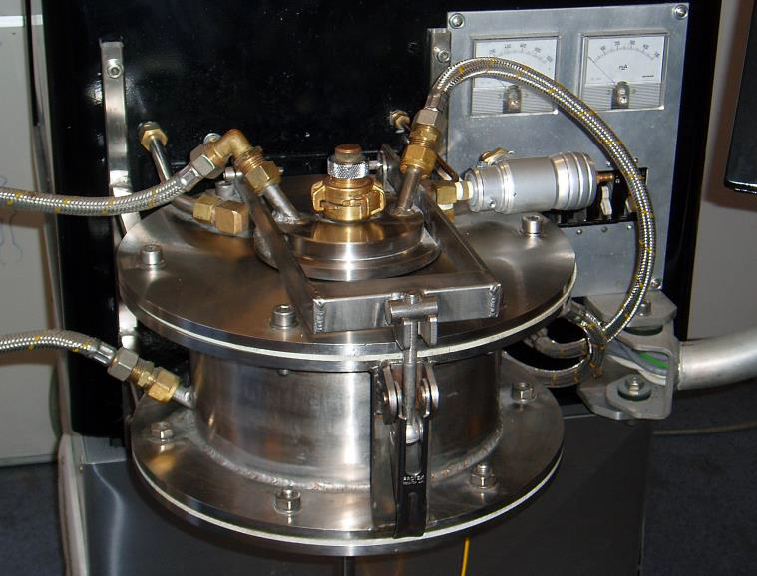
\includegraphics[width=\textwidth]{Ex_LAWS_Induction_Casting.png}
		\caption{}
		\label{fig:LawsCasting}
	\end{subfigure}
	%Image 4
	\begin{subfigure}[htbp]{0.375\textwidth}
		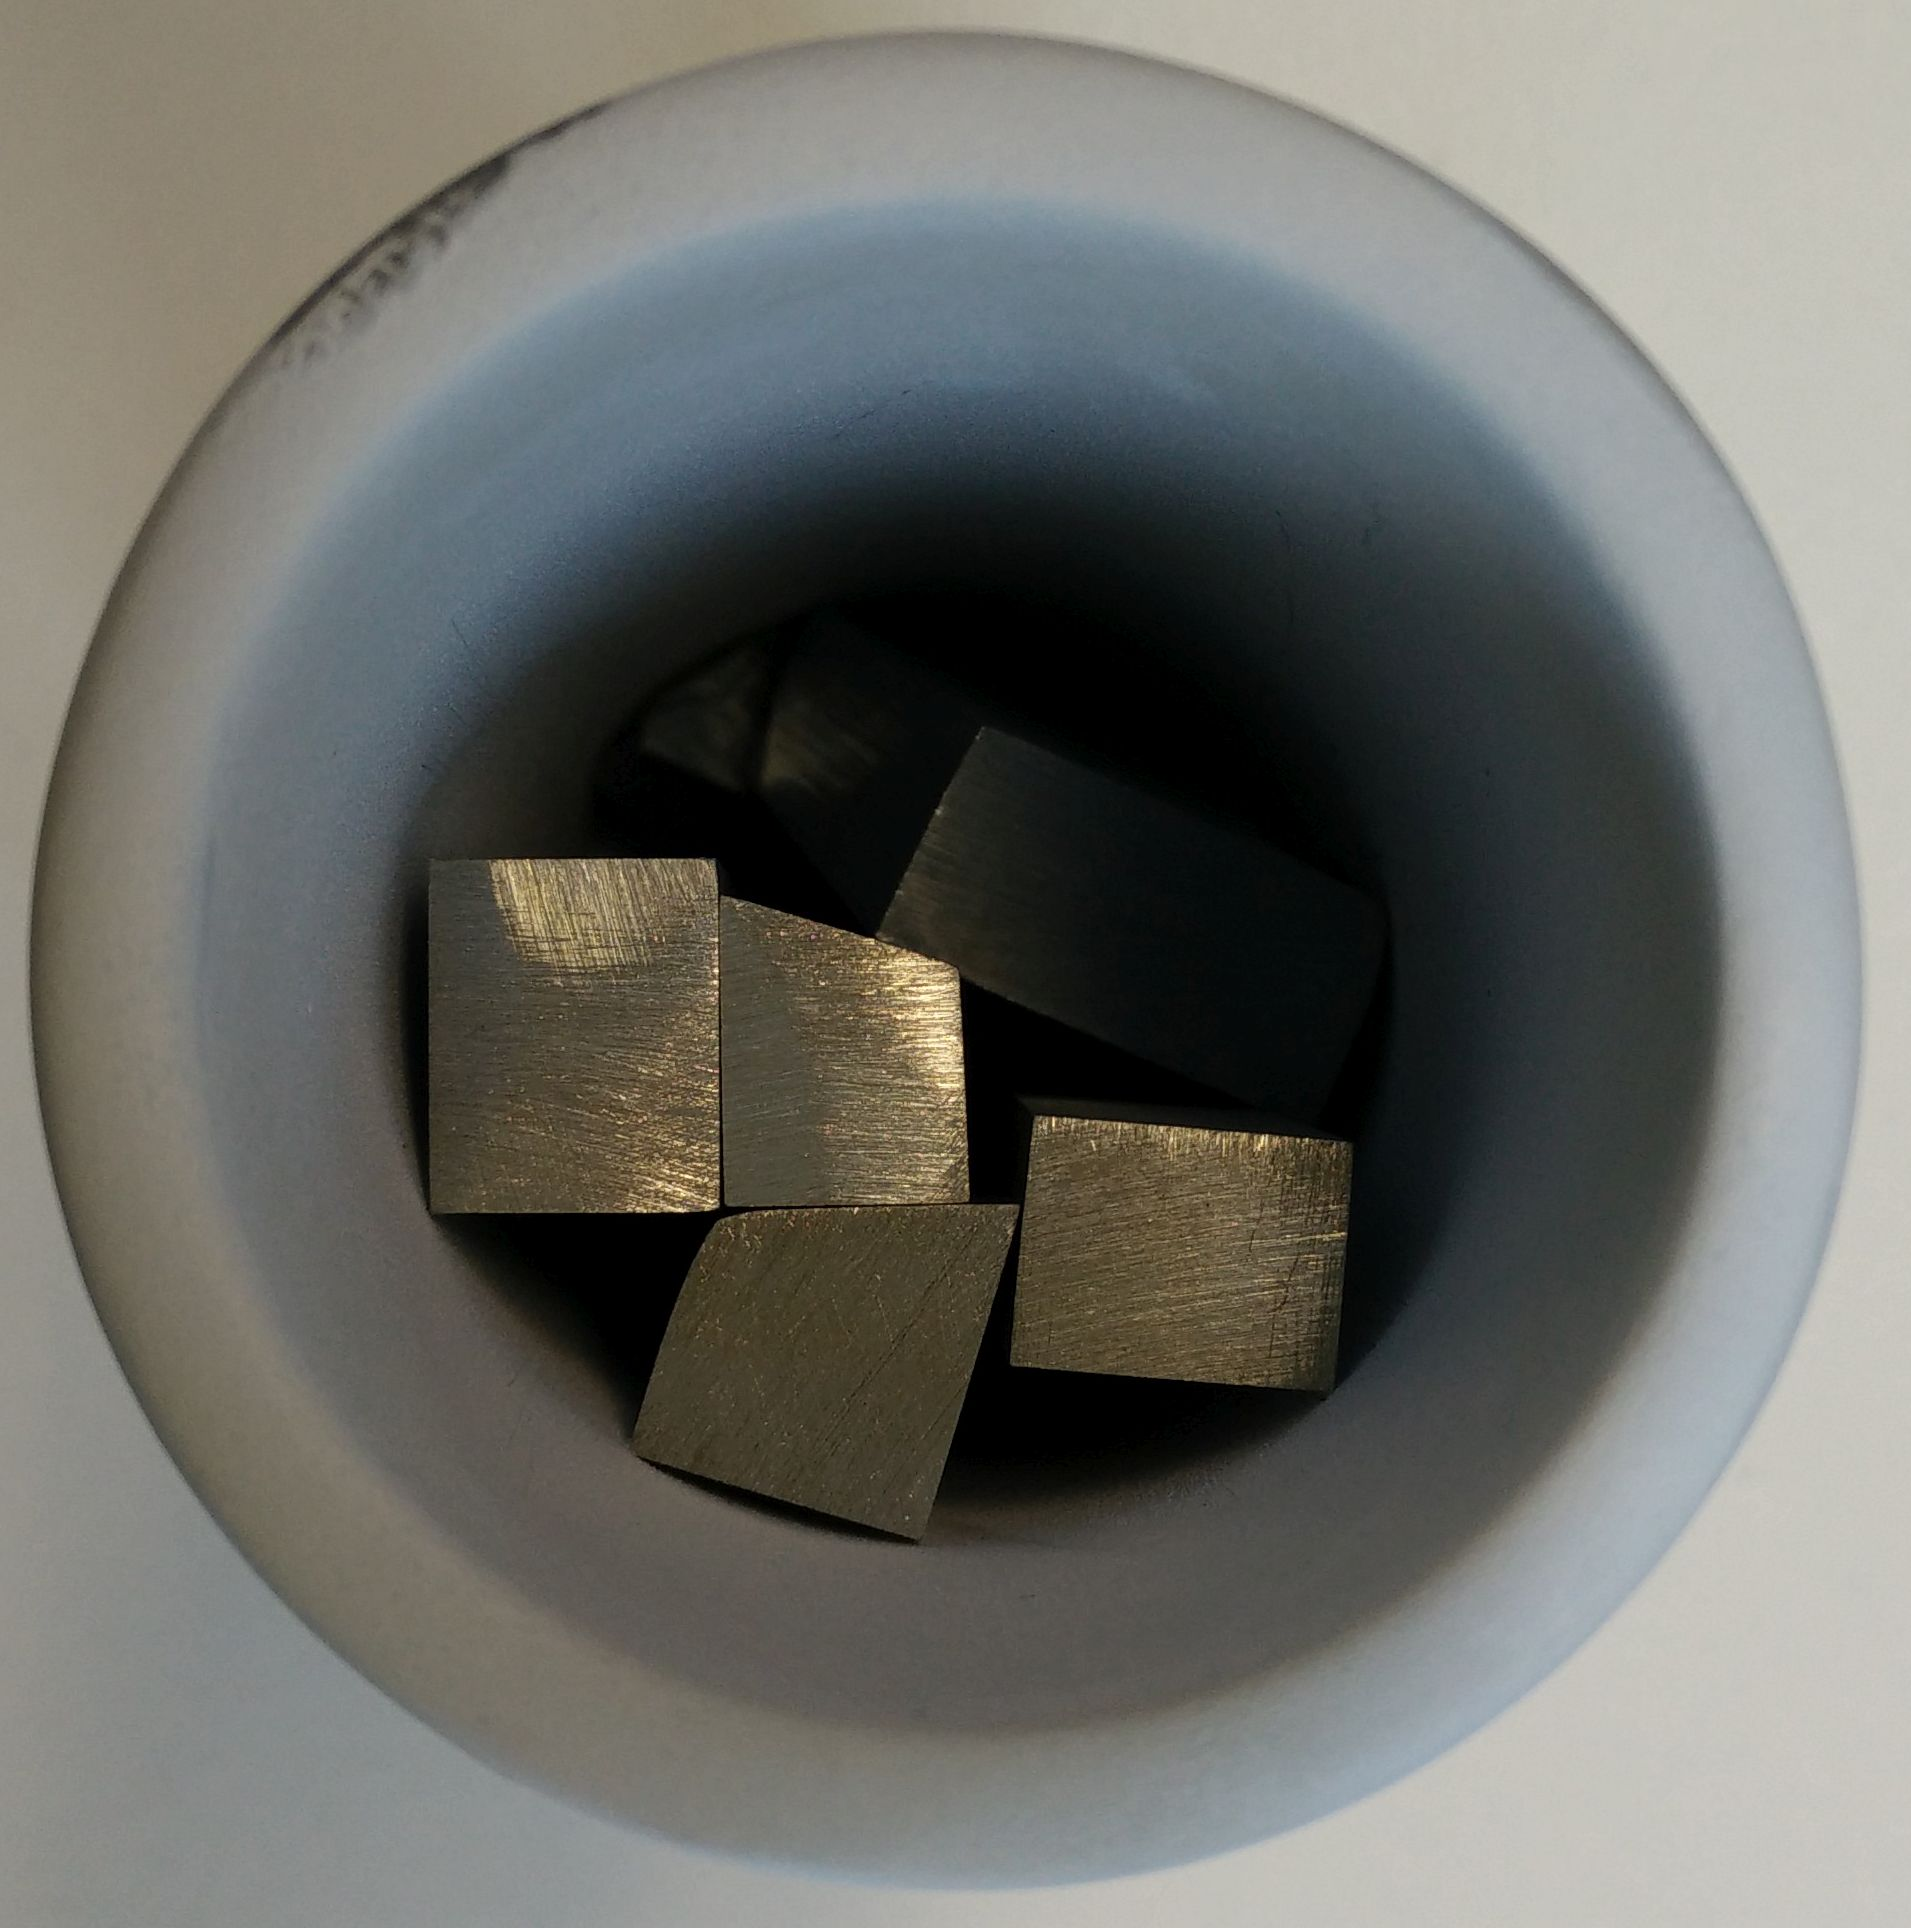
\includegraphics[width=\textwidth]{Ex_Crucible_Charge.jpg}
		\caption{}
		\label{fig:CrucibleCharge}
	\end{subfigure}
	%Image 2
	\begin{subfigure}[htbp]{0.41\textwidth}
		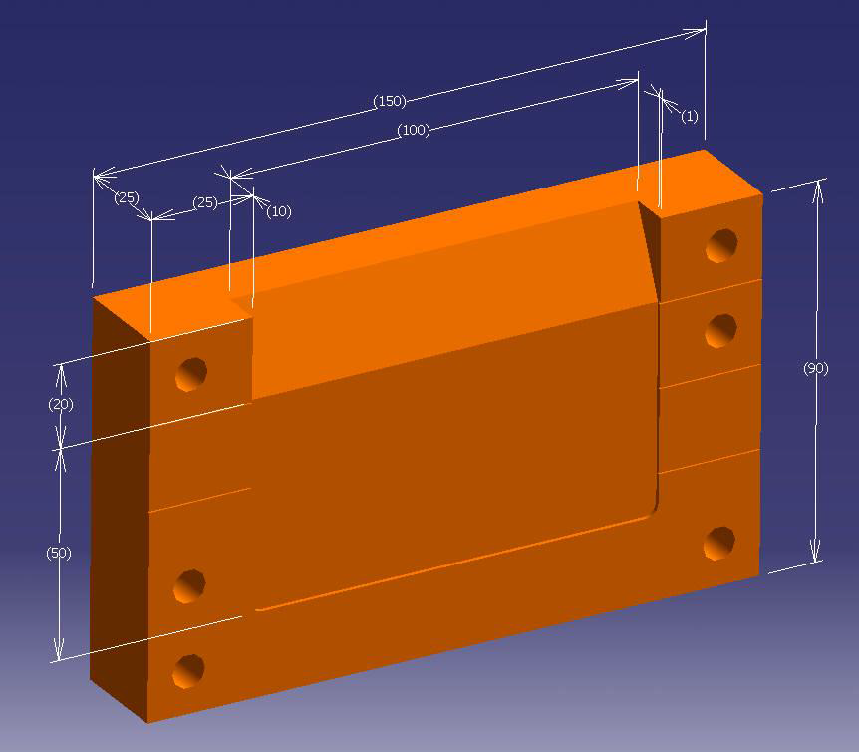
\includegraphics[width=\textwidth]{Ex_Laws_Copper_Mould.png}
		\caption{}
		\label{fig:LawsMould}
	\end{subfigure}
	%Image 3
	\begin{subfigure}[htbp]{0.49\textwidth}
		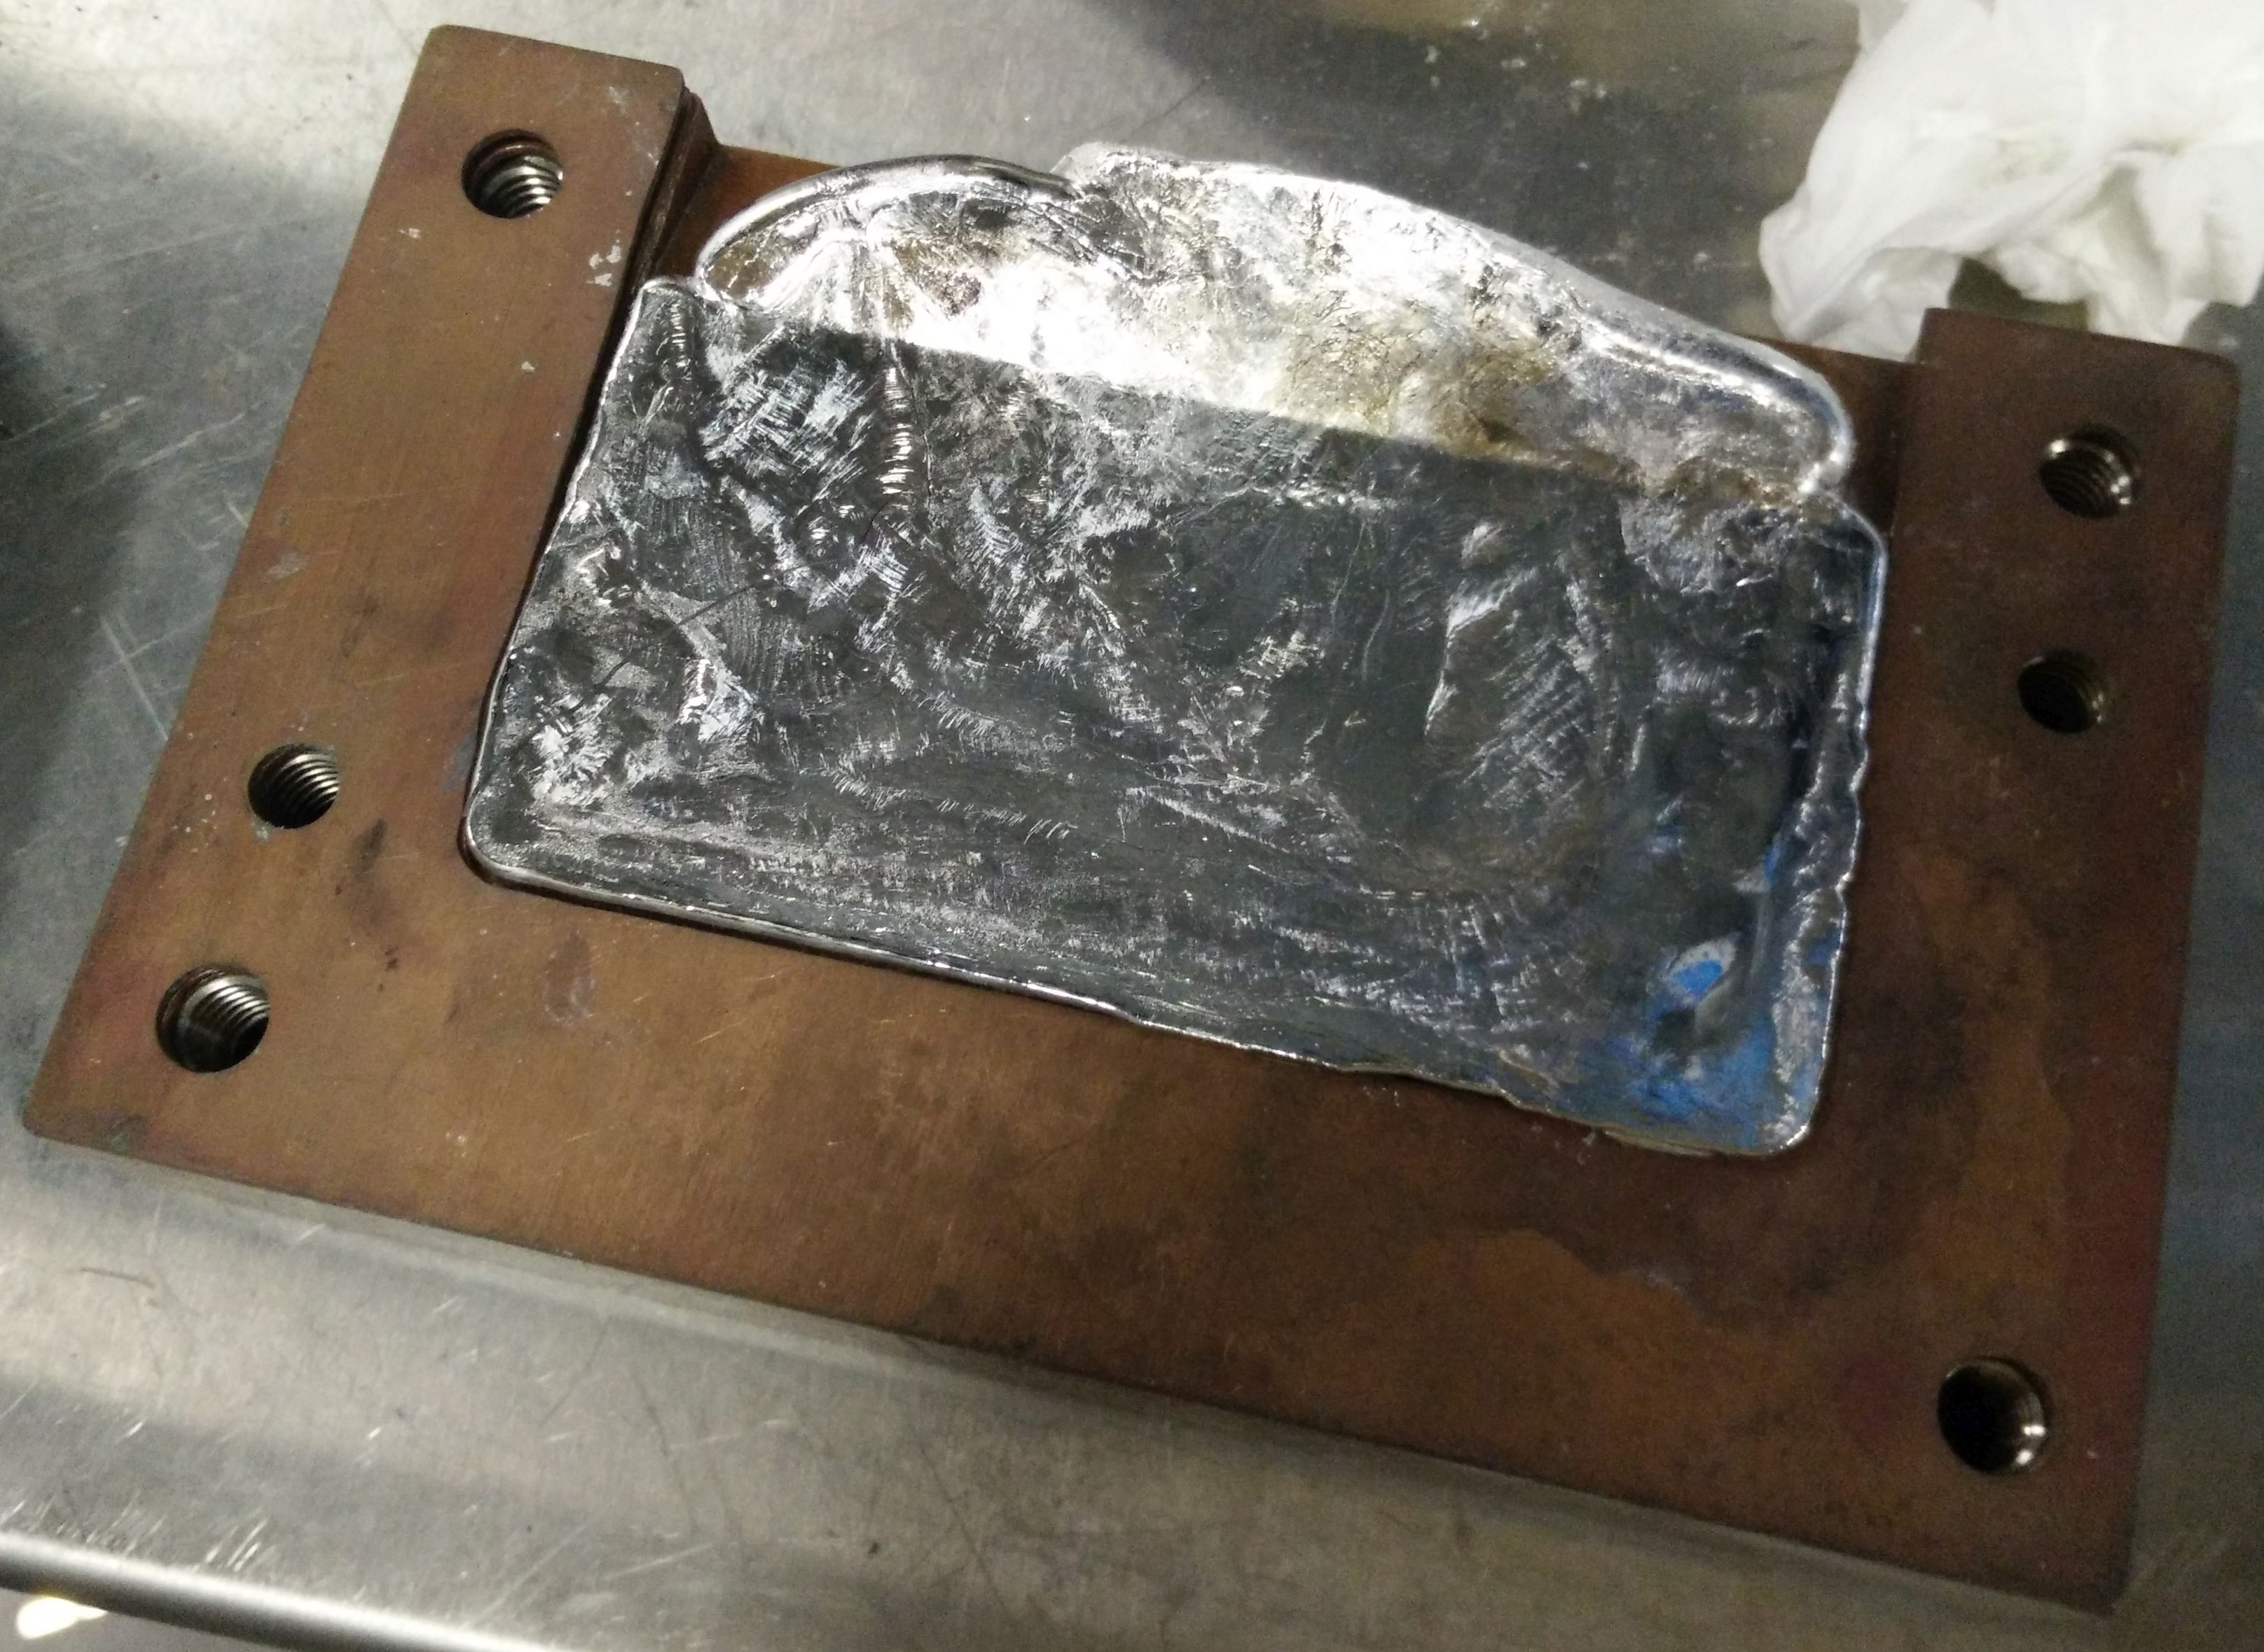
\includegraphics[width=\textwidth]{Ex_Mould_Cast_Plate.jpg}
		\caption{}
		\label{fig:FilledMould}
	\end{subfigure}
	\caption[(a) Inducting casting chamber. (b) Boron nitrate coated graphite crucible with Mg and Zn ingot charge. (c) 3D schematic of copper plate mould with dimentions. (d) Cast \MgZnCa~ master alloy plate within mould.]{(a) Inducting casting chamber. (b) Boron nitrate coated graphite crucible with Mg and Zn ingot charge. (c) 3D schematic of copper plate mould with dimentions. (d) Cast \MgZnCa~ master alloy plate within mould. (a) and (c) reproduced from \cite{Laws2007}.}%global caption
	\label{fig:Induction}
\end{figure}

\subsection{Final Shaping}
\subsubsection{Riser Removal} \label{sec:RiserRemoval}
Once master alloy plate was cast the riser was removed. The plate was mounted in a polymer grip vice and the riser carefully cut off with a 24 or 32 \acrshort{tpi} hacksaw. Paper was placed under the vice grips to capture the dust for later analysis (Figure \ref{fig:Vice}).

\subsubsection{Target Extraction}
The target was extracted from the plate by a notched $32~ mm$ diameter diamond holesaw (Suttontools) on a Hercus Sales (W2) drill press at 360 \acrshort{rpm} with a bore rate of approximately $15~ mm/hr$. The plate was mounted in a polymer grip horizontal vice on top of cut plywood for dampening, and placed in a drip tray. A constant stream of lubricating distilled water was supplied by a standard spray bottle (Figures \ref{fig:DrillBit} and \ref{fig:DrillPress}).

\subsubsection{Target Rounding}
The target was then shaped to a nominal $1~ in$ ($25.2 - 25.4~ mm$) diameter disk by removal of excess circumferential material. Large sections were removed by hacksaw as outlined in Section \ref{sec:RiserRemoval}, with finer shaping accomplished by linishing operations. Target roundness was checked throughout by comparing with a 2 Euro or washer template, $25.75~ mm$ and nominal $25.4~ mm$ diameter respectively. Final nominal target diameter was confirmed by vernier caliper measurement (Figure \ref{fig:TargetEuro}).  

\subsubsection{Target Polishing}
The target was progressively manually polished with light pressure on glass plate in a figure eight pattern with flowing lubricating water. Targets were polished on both sides and rotated through small angles every couple seconds to ensure a consistent flat surface. The grit progression was 320, 800, 1200, and 4000 with target washing between all stages. After 800 and higher grit stages the target was ultrasound cleaned for 1 minute in soap and water. Polishing wheels were not used because they produce a less consistent flat surface and targets require high surface tolerance to fire within the sputtering gun. Target flatness was checked by micrometre, with nominal variation between the two opposing surfaces being less than 1\% the target diameter, about $0.254~ mm$. 

%single image
\begin{figure}[htbp]
	\centering
	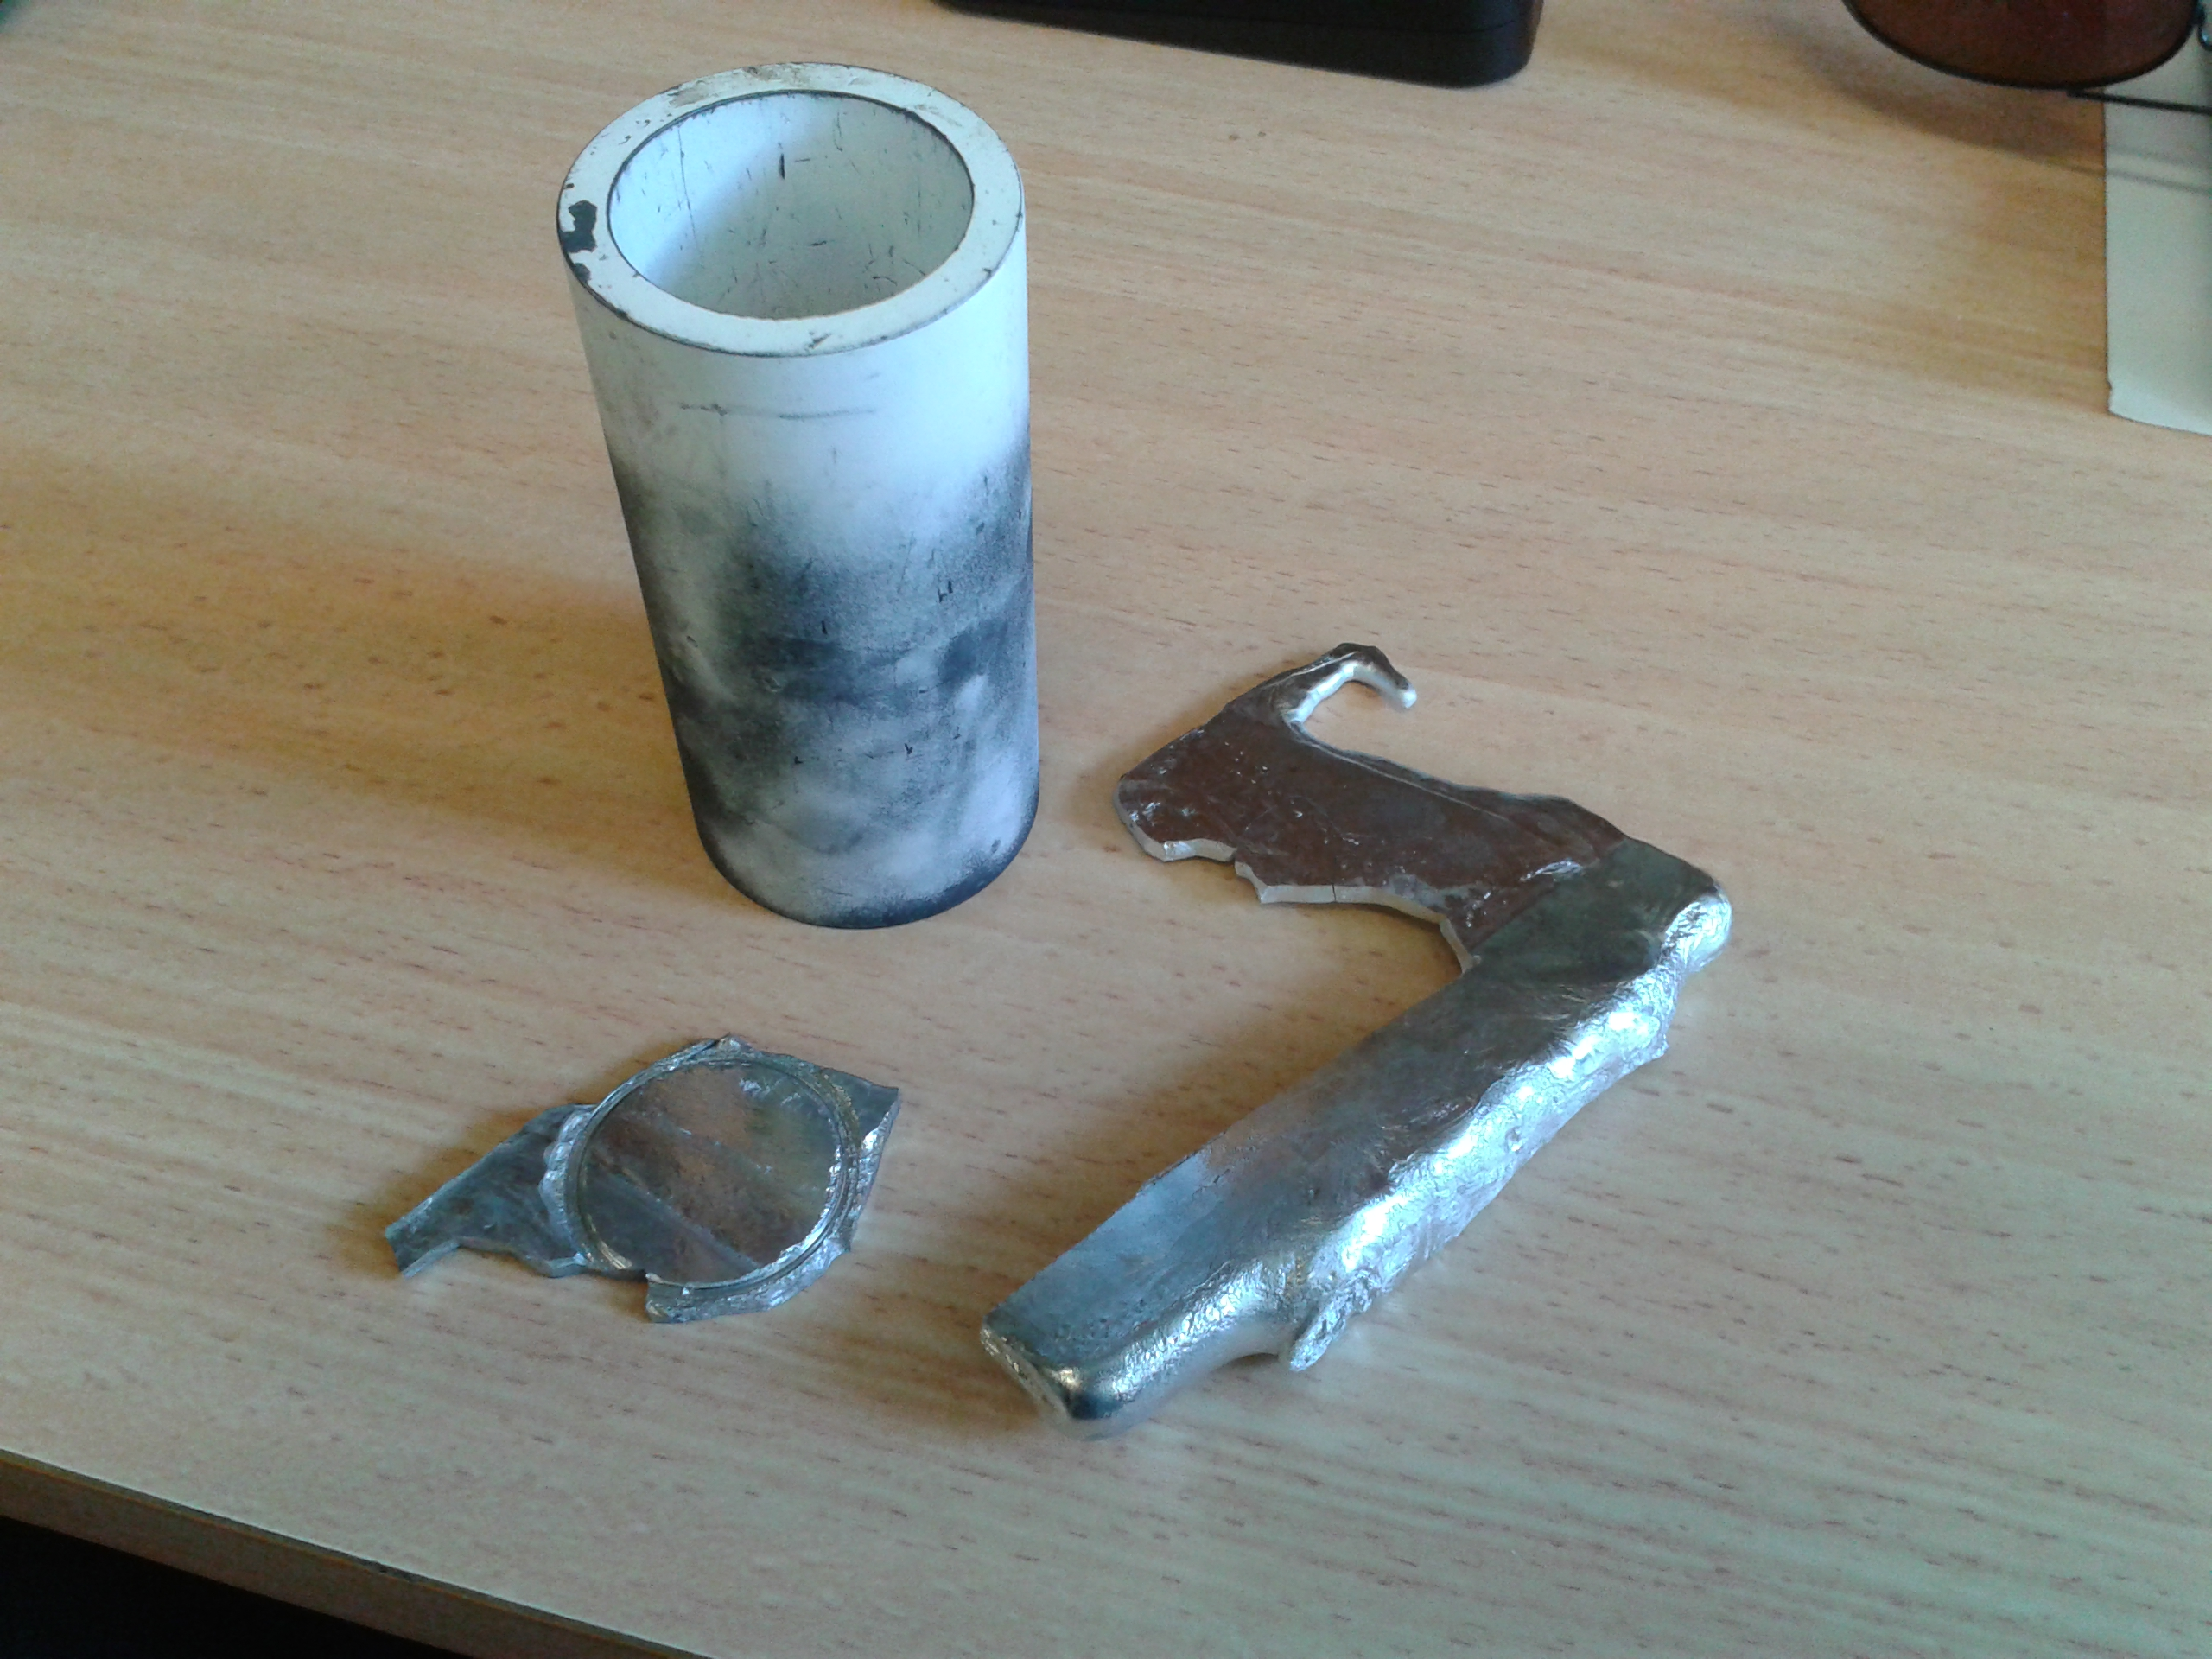
\includegraphics[width=0.75\textwidth]{Ex_CruciblePlateRiserRoughtarget.png}
	\caption{(a) Boron nitrate coated graphite crucible for induction furnace melting of alloys, (b) Cracked \MgZnCa~ master alloy plate, (c) Riser cut free from main casting, and (d) Drilled and partly shaped target.}
	\label{fig:CrucibleShaping}
\end{figure}

%code to put 4 images side by side in a figure
\begin{figure}[htbp]
	\centering
	%Image 1
	\begin{subfigure}[htbp]{0.49\textwidth}
		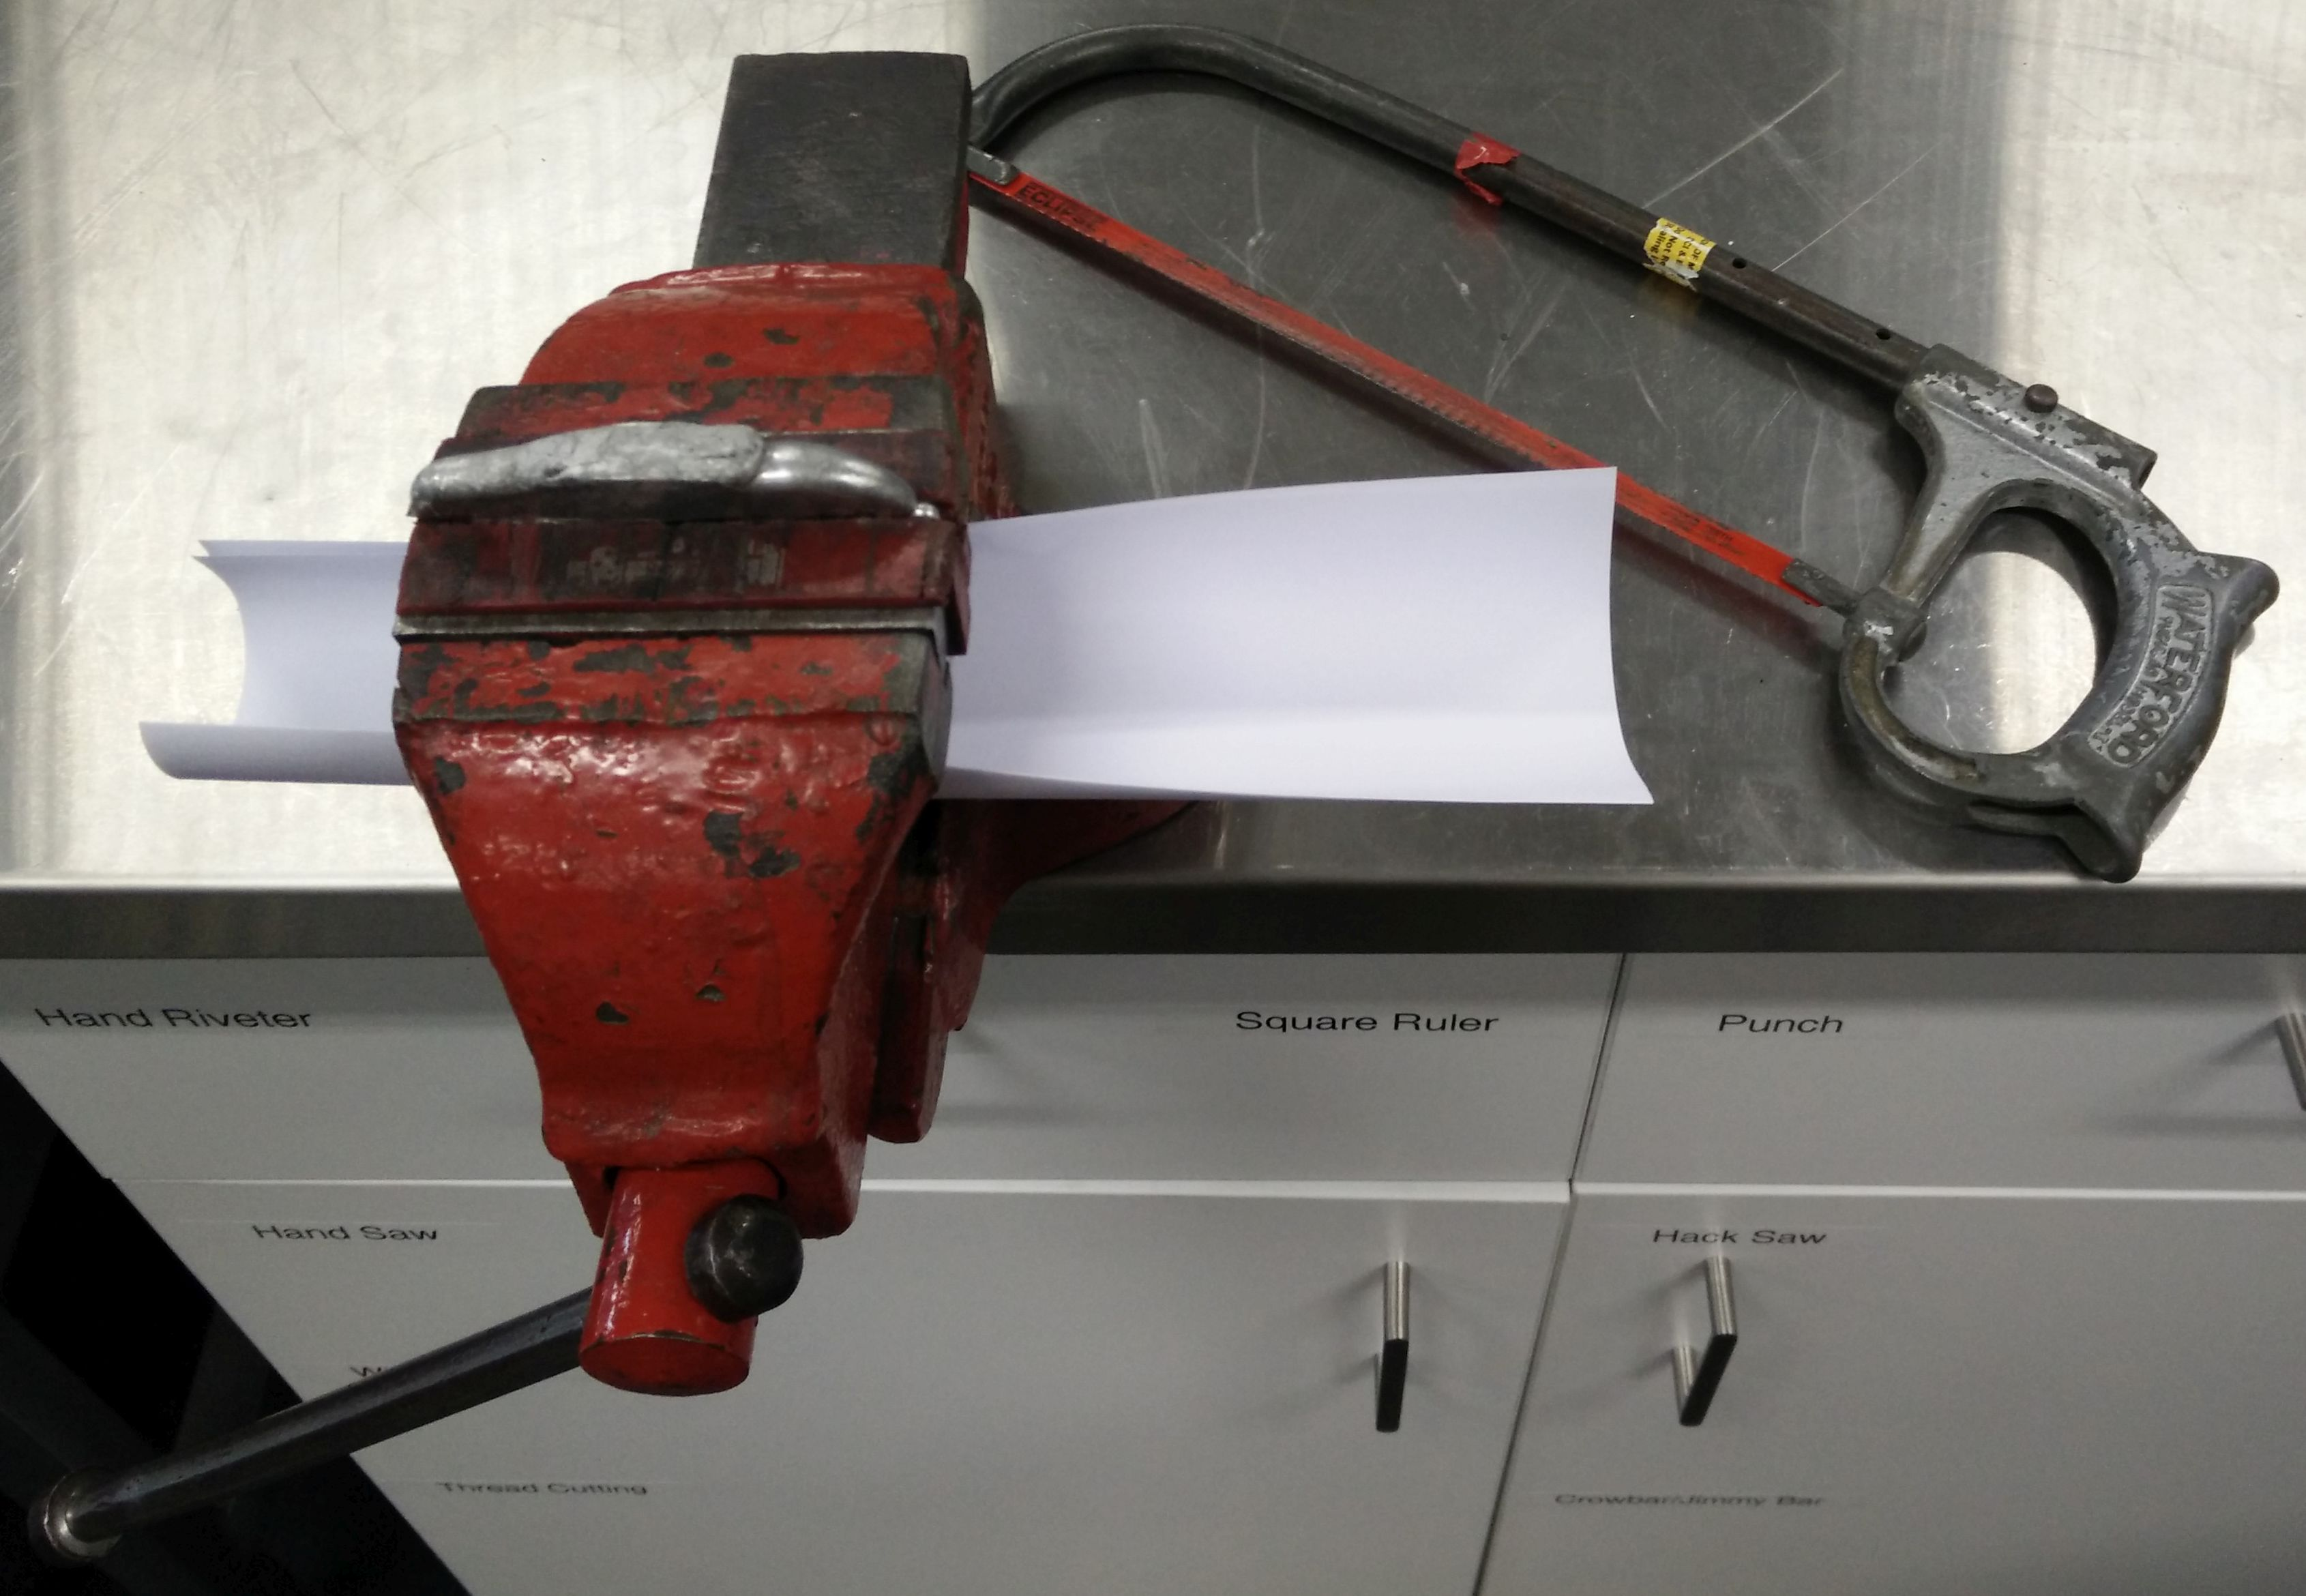
\includegraphics[width=\textwidth]{Ex_Vice_Hacksaw.jpg}
		\caption{}
		\label{fig:Vice}
	\end{subfigure}
	%Image 2
	\begin{subfigure}[htbp]{0.38\textwidth}
		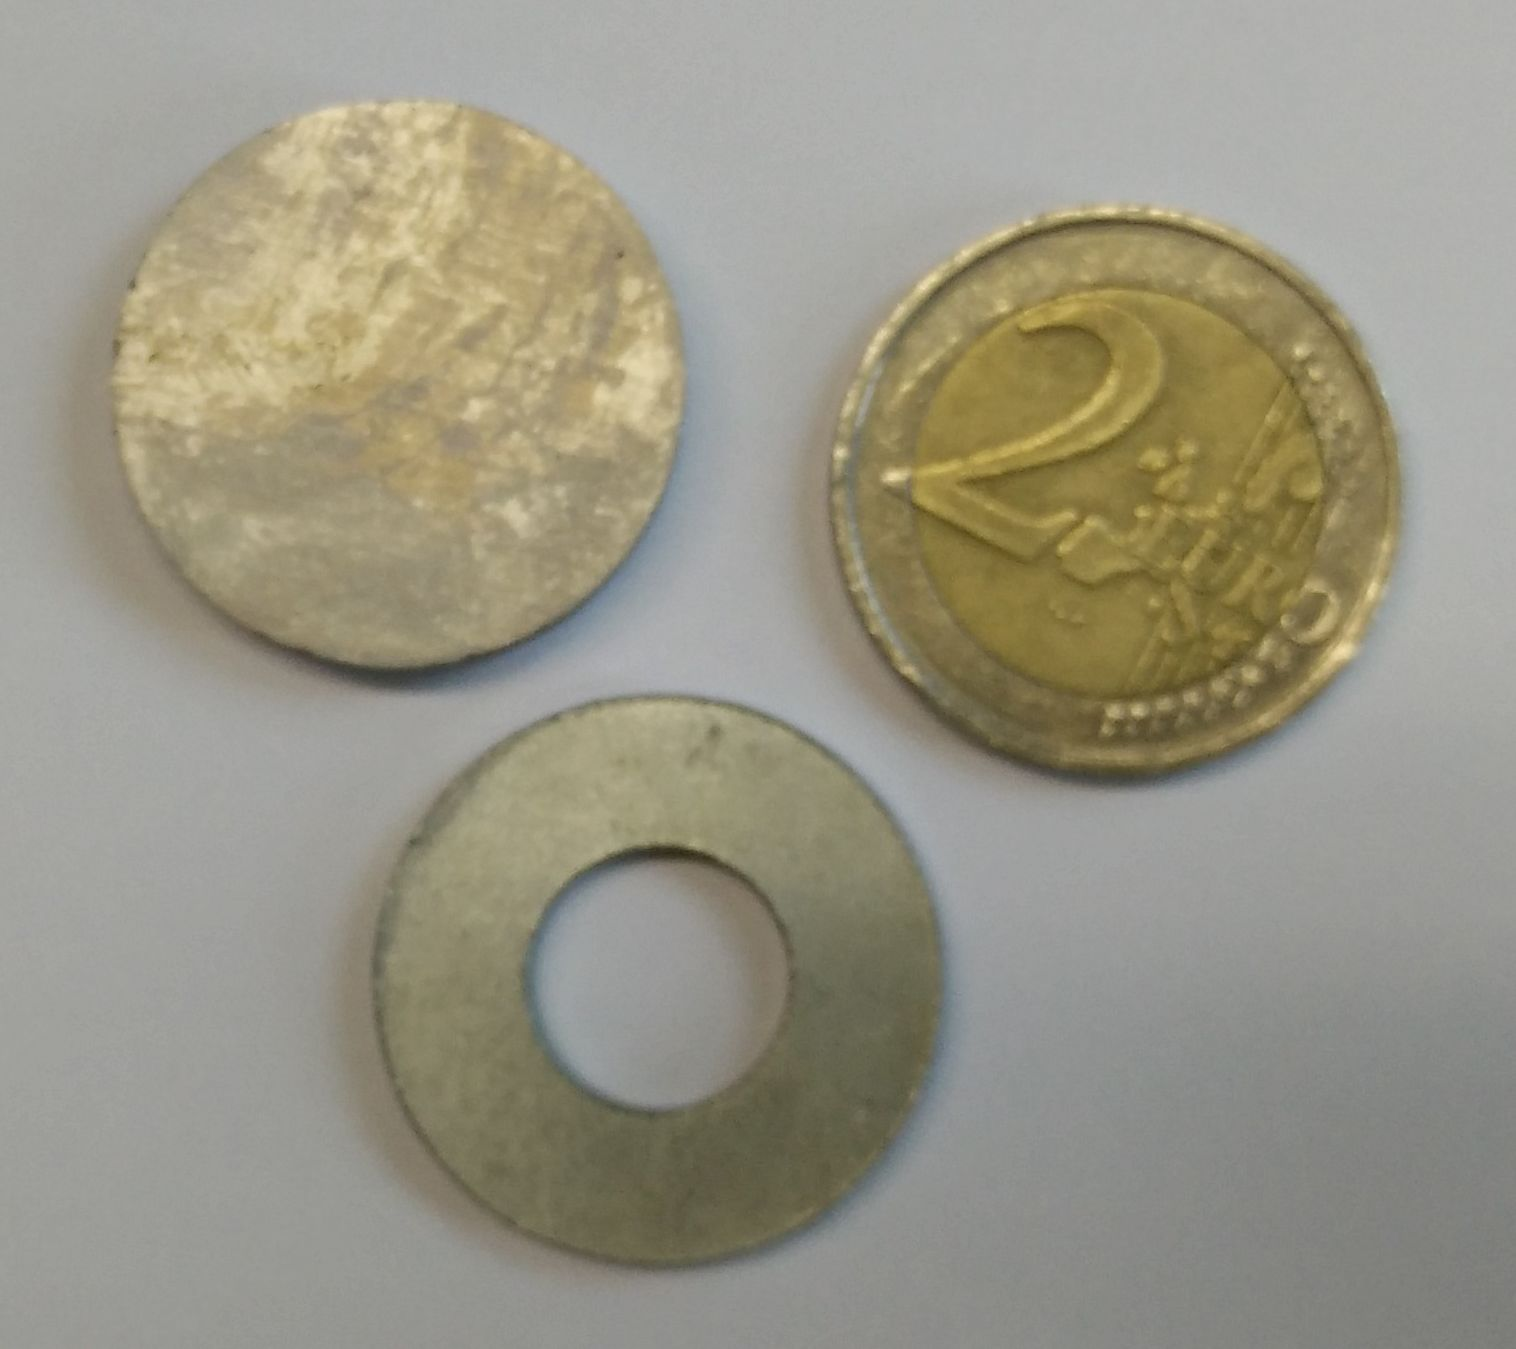
\includegraphics[width=\textwidth]{Ex_Target_Euro.jpg}
		\caption{}
		\label{fig:TargetEuro}
	\end{subfigure}
	%Image 3
	\begin{subfigure}[htbp]{0.275\textwidth}
		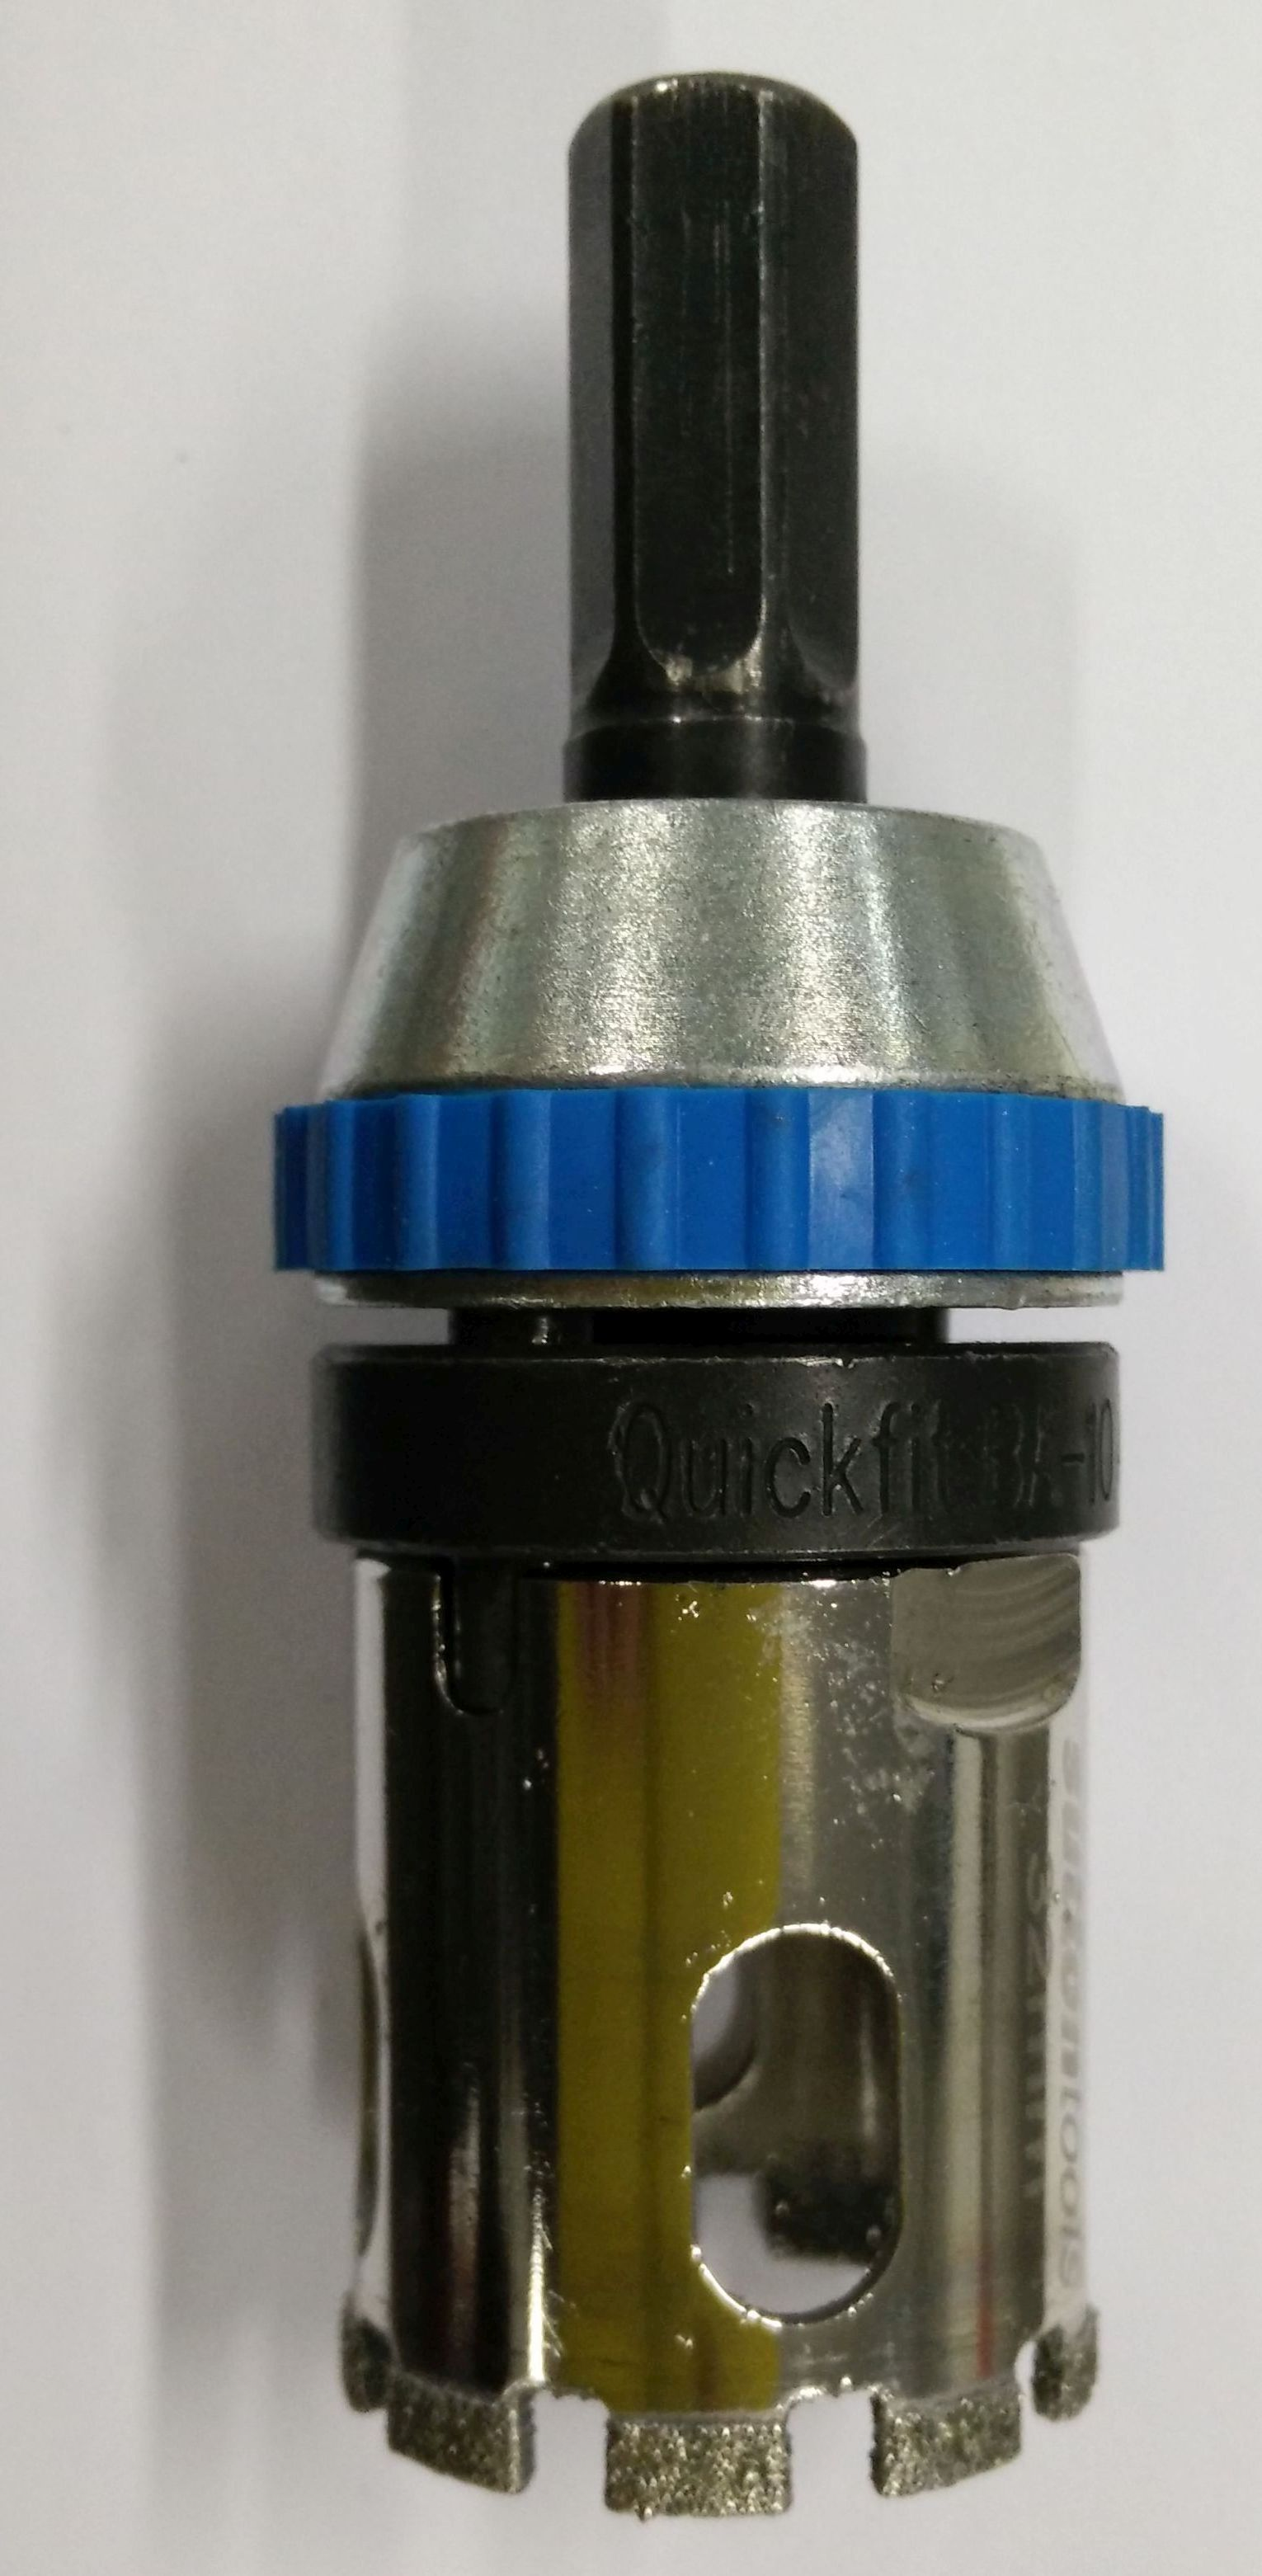
\includegraphics[width=\textwidth]{Ex_Drill_Bit.jpg}
		\caption{}
		\label{fig:DrillBit}
	\end{subfigure}
	%Image 4
	\begin{subfigure}[htbp]{0.30\textwidth}
		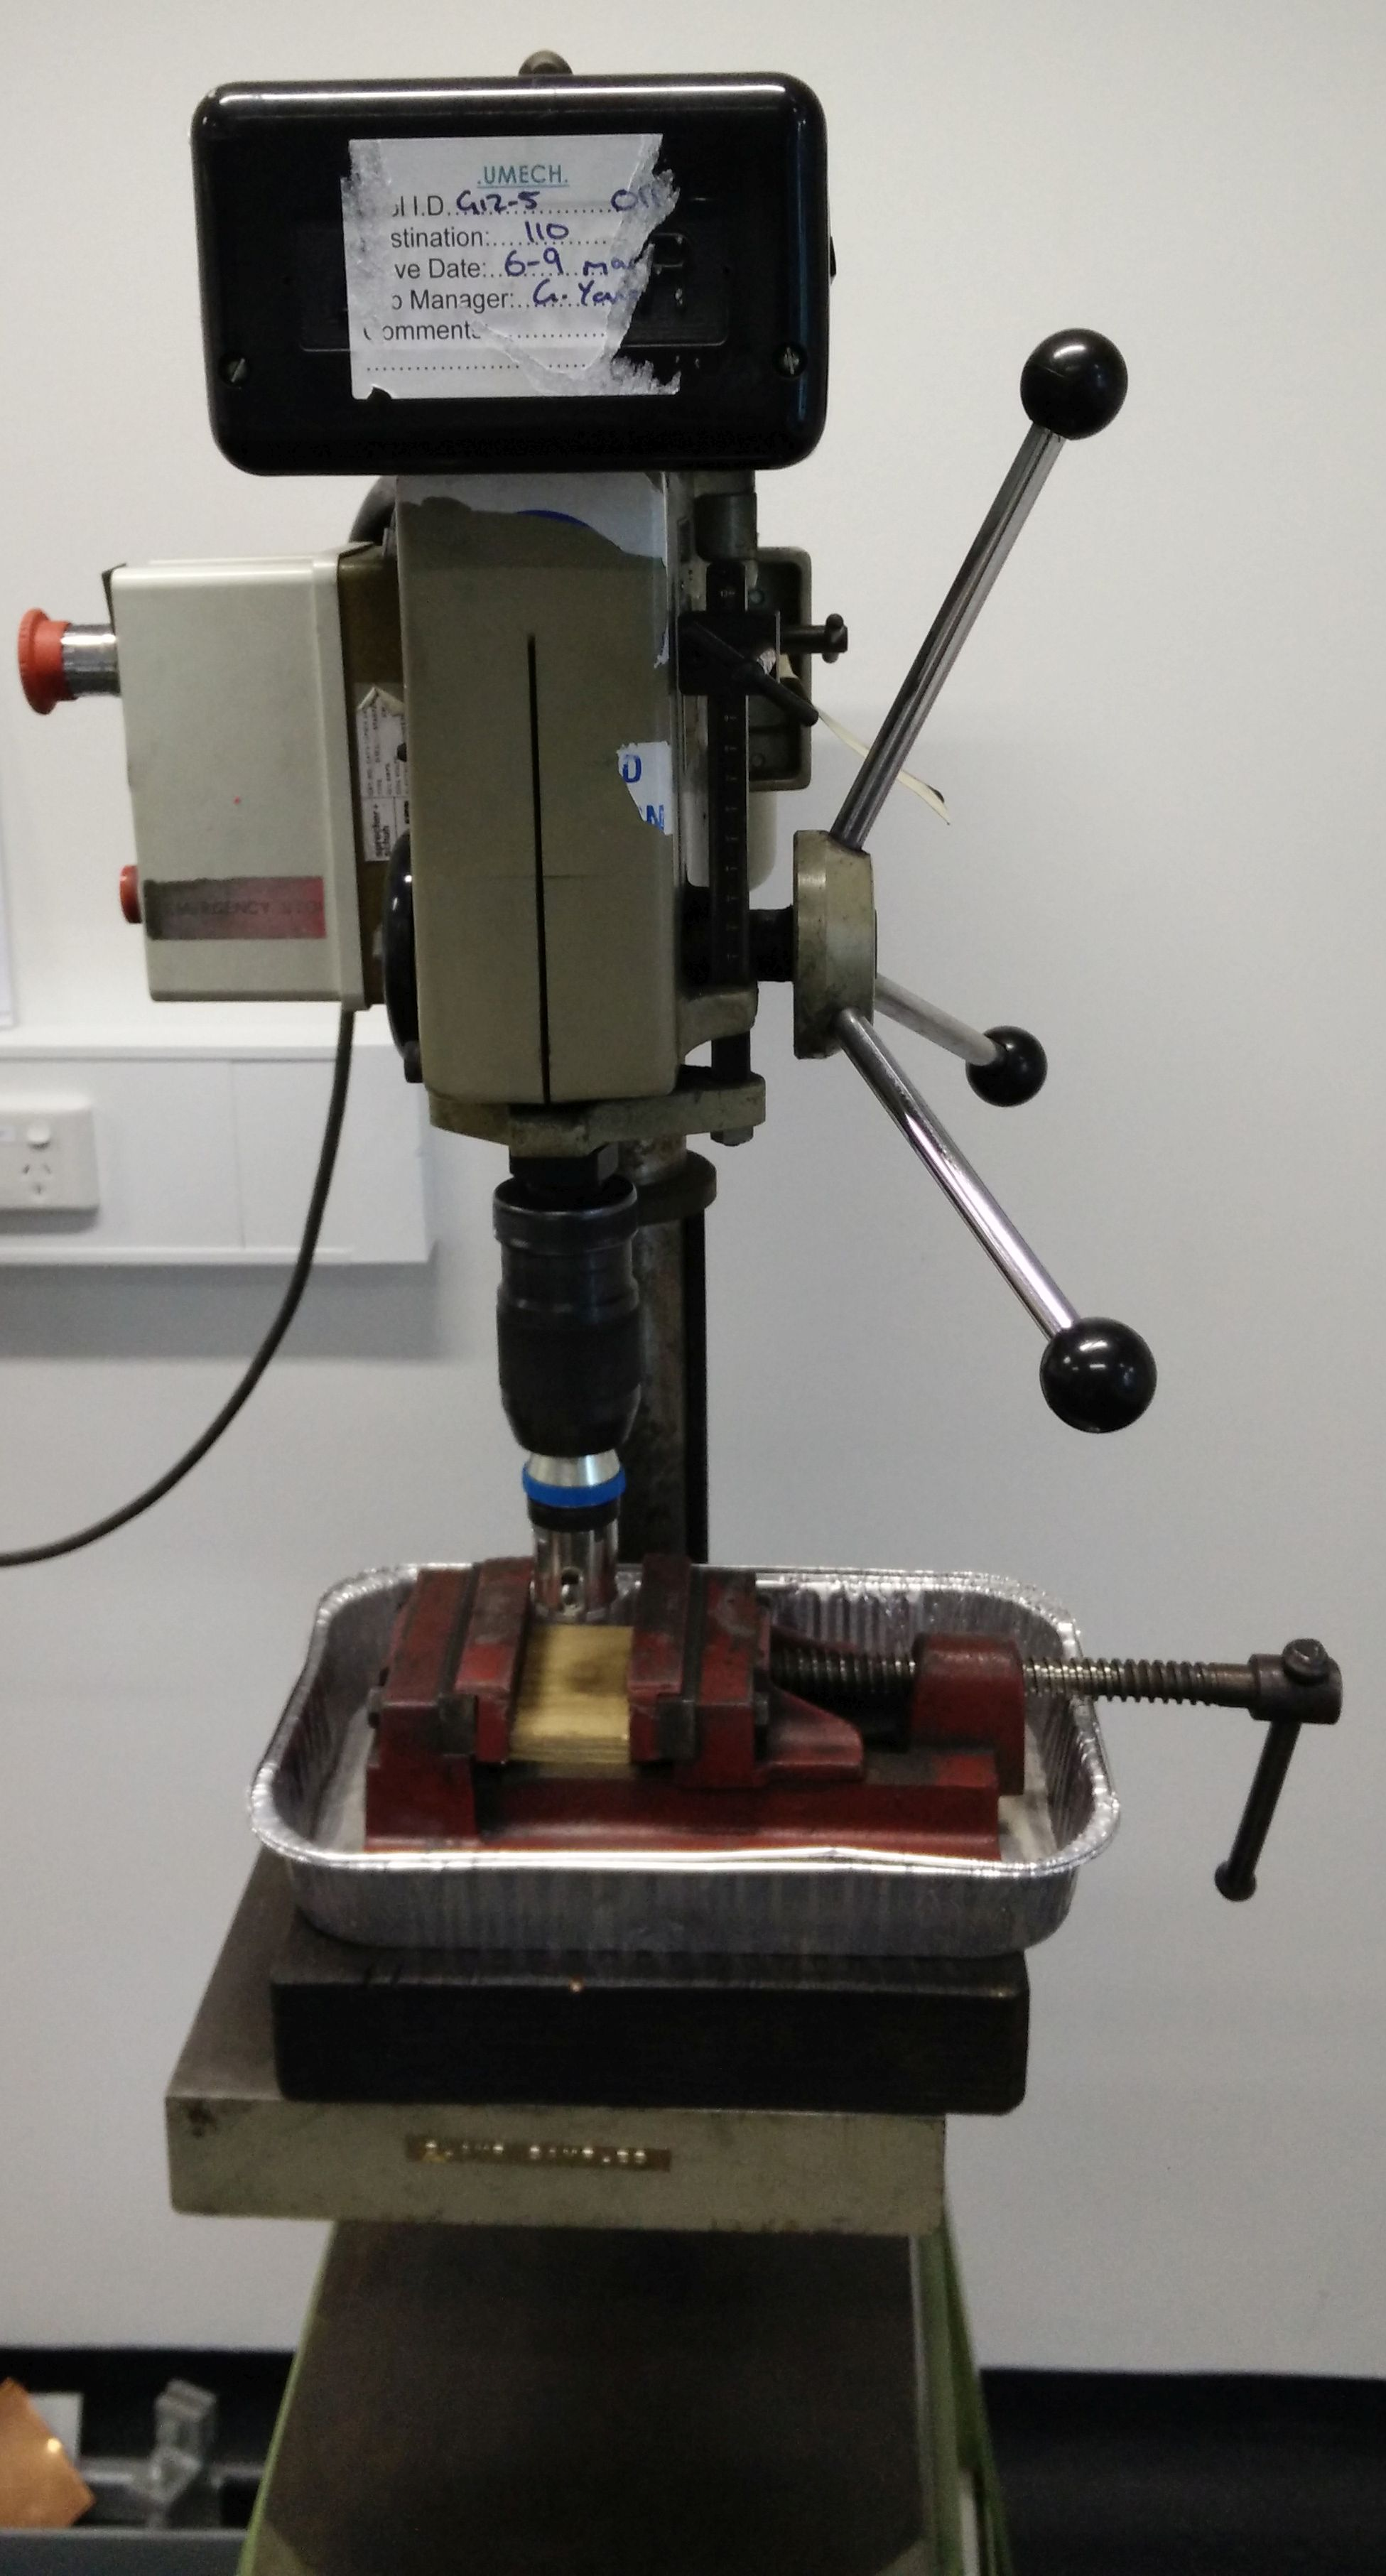
\includegraphics[width=\textwidth]{Ex_Drill_Press.jpg}
		\caption{}
		\label{fig:DrillPress}
	\end{subfigure}
	\caption{(a) Polymer grip vice clamping plate below riser with 32 \acrshort{tpi} hacksaw. (b) Fully shaped, unpolished target with 2 Euro and washer template. (c) Notched $32~ mm$ diameter diamond holesaw. (d) Drill press, holesaw, horizontial vice with polymer grips, plywood damper and drip tray for target extraction.}%global caption
	\label{fig:ShapingEquipment}
\end{figure}

\section{Crystalline Target Manufacture} \label{sec:CrystalTargetManufacture}
Fully crystalline targets were later manufactured as they could be produced more quickly and found to provided similar deposition results to semi-crystalline targets. Manufacture was as per Section \ref{sec:TargetManufacture} except where noted.

\subsection{Induction Furnace Melting}
\subsubsection{Melt Cycle}
As before prepared crucible charges were sealed in the induction furnace chamber, evacuated and purged with Ar (99.997 vol.\% purity) five times before starting a continues circulating Ar flow. The crucible charge was induction melted at 700\degree C for a couple minutes and stirred with a tungsten rod. The melt was then partially solidification at 385\degree C, remelted and stirred at 650\degree C, partially re-solidification at 385\degree C, and remelted and stirred again at 650\degree C. The melt was then cooled and held for 30 seconds at casting temperature of $450$\degree C. It was then stirred and removed from the melt chamber by the incorporated raising bar. 

\subsubsection{Gravity Casting}
For naturally cooled gravity casting the melt was manually poured into a prepared copper cylinder mould. The casting cavity diameter is $25.6~ mm$, with a depth of $60~ mm$, and no riser allowing for a casting volume of approximately $30~ cc$. The mould was prepared by cleaning with lint free paper, polishing with Brasso \textcopyright, and wiping clean again with the paper.

\subsection{Final Shaping}
Crystalline Targets have a different shaping processes from Section \ref{sec:TargetManufacture}.

\subsubsection{Sectioning of Targets}
Once cast the top and bottom quarter of the casting was removed on an auto-cutter (Struers Accutom-50) fitted with a diamond blade (Leco $4"~ X~ 0.012"~ X~ 1/2"$) at a feed rate of no more than $0.02~ mm/s$ at $2000$ \acrshort{rpm} with medium force. This removed the inconsistencies due to the quick initial cooling of the pour, and feeding of the final melt. The remaining, consistent casting was then sectioned into nominally $3.85~ mm$ thick targets.

\subsubsection{Target Rounding}
Sectioned targets were slightly oversized and quickly shaped to a nominal $1~ in$ ($25.2 - 25.4~ mm$) diameter disk by linishing operations and confirmed by vernier caliper measurement.

\subsubsection{Target Polishing}
The target was progressively manually polished as before.

\clearpage

\section{DC Magnetron Sputtering}
\subsection{DC Magnetron Sputtering Equipment}
The thin films were deposited by an in house \acrshort{dc} magnetron sputtering facility (Figure \ref{fig:CaoSputtering}). This facility has a maximum power of 50 W, with a working gas of ultra-high purity Ar (99.999\%). The sputtering gun nominal target diameter is $25.4~ mm$ ($1~ in$). The working distance between target and substrate holder is \hl{$8~ cm$}. The chamber can achieve a base vacuum pressure of at least \hl{$10^{-2}~ Pa$}, and a working Ar pressure of at least \hl{$2~ Pa$} at constant flow rate of \hl{$2~ cm^{3}/s$}. The chamber has direct access and a large deposition area, allowing for batch processing of multiple substrates simultaneously.

%single image
\begin{figure}[htbp]
	\centering
	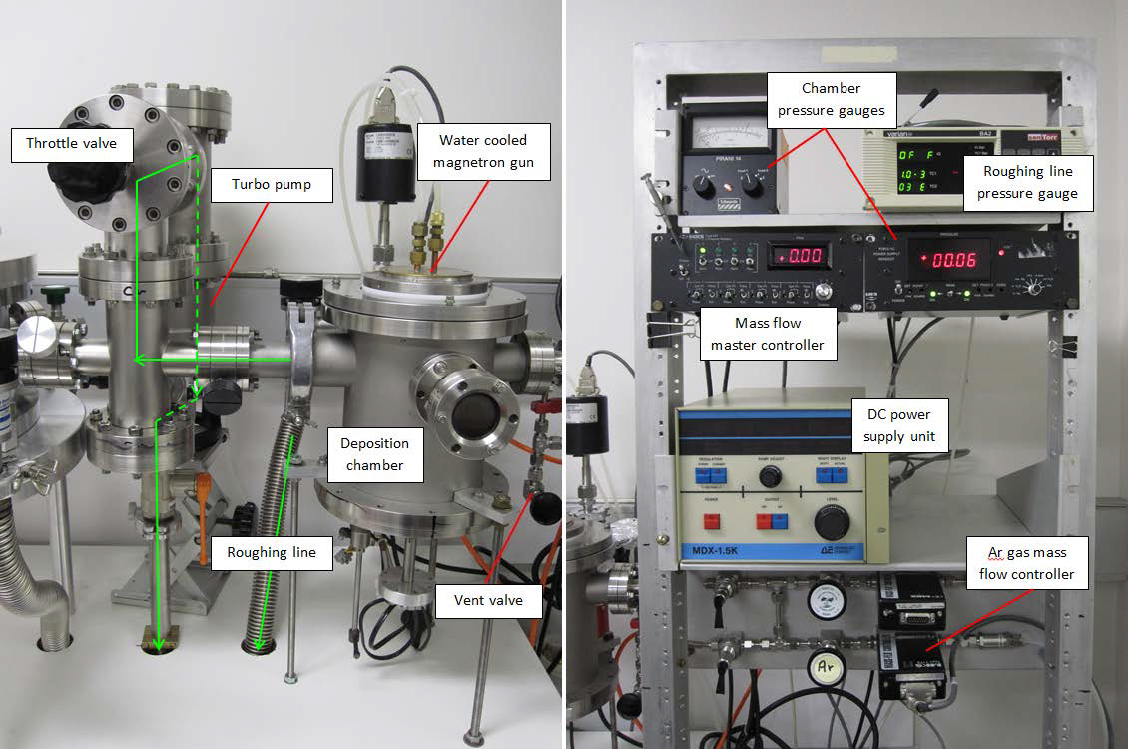
\includegraphics[width=0.75\textwidth]{Ex_Cao_SputterMachine.png}
	\caption[In house \acrshort{dc} magnetron sputtering facility.]{In house \acrshort{dc} magnetron sputtering facility. Reproduced from \cite{Cao2013}.}
	\label{fig:CaoSputtering}
\end{figure}

\subsection{Depostion of Thin Films}
A target was affixed in the sputtering gun mount by applying \hl{thermal gel} to one side for coincident contact. The desired substrate was position on the sample stage within the chamber and the chamber sealed. The chamber was evacuated to the desired base pressure, and then backfilled to the desired working Ar pressure. Coincident Ar pressure was maintained by a constant flow of Ar gas. This was necessary because the number of Ar$^{+}$ cations increases with chamber pressure, and accordantly increases the rate of deposition \cite{Ozeki2002}. Before deposition the targets were prepared by a pre-sputter to remove contamination and oxides from their surface. During this stage the substrates were protect by a shield positioned over the sample area preventing deposition.

The \glspl{tfmg} were deposited onto room temperature substrates, and \glspl{smg} onto elevated temperate substrates. The elevated substrate temperatures were achieved and controlled by a hot plate and K-type thermocouple.

The initial \gls{tfmg} sputtering parameters were based on Liu, et al. \cite{Liu2012} work on \ZrCuNiAl~ film refinement, and the \gls{smg} parameters were based on Yu, et al. \cite{Yu2013} and Aji, et al. \cite{Aji2013} work on \ZrCuAl~ and \ZrCuNiAl~ \gls{smg} films respectively. These parameters were refined by appropriate step sizes as required to suit the examined MgZnCa biocompatible systems. 

%table
\begin{table}[h]
	\centering
	\begin{tabular}{ l l l }
		\toprule
		Nominal Sputtering Parameters: & \acrshort{tfmg} & \acrshort{smg} \\
		\midrule
		Base Camber Pressure: & $3 \times 10^{-4} - 10^{-2}~ Pa$ & $5 \times 10^{-5} - 10^{-4}~ Pa$ \\
		Deposition Ar Pressure:	& $0.3 - 3.0~ Pa$ & $5\times 10^{-2} - 0.3~ Pa$\\
		Deposition Power Range:	& $30 - 50~ W$ & $30 - 50~ W$\\
		Max Deposition Rate: & $3.3~ nm s^{-1}$ & $1.4~ nm s^{-1}$ \\	 
		Substrate Deposition Temperature: & \acrshort{rt} & $0.7 - 0.8$ \acrshort{Tg} \\
		\bottomrule
	\end{tabular}
	\caption{Nominal Sputtering Parameters}
	\label{tab:NomSputterParameters}
\end{table} \todo{Probably will be much closer to the 50 W end (Jake topped out at 55 W).
MgCaZn has more light elements near Ar than ZrCuNiAl.
Therefore expect greater deposition efficiencies and to not require as much power.
ZrCuNiAl used 50 – 150 W, but we cannot get power that high unless we use 3 inch targets (not practical).} 	

\subsection{Target Lifespan}
Each target was expected to be able to deposit approximately $10 - 15~ \mu m$ of total film thickness onto a substrate, which was about an hour of deposition at rate of 3.3nm/s. After full deposition the targets were no longer usable and were stored for analysis or disposed. 

\section{Examined Substrates} 
The thin films will be deposited onto four different substrates for examination; silicon wafer, water soluble substrate, \gls{bmg} substrates, and \gls{pcl} scaffold substrates.

\subsection{Silicon Wafer Substrate}
Thin films are easily and readily deposited onto un-doped (100) silicon wafer with minimal difficult. This substrate allows film properties to be easily examined with minimal influence from the substrate (I.E. film amorphousness can be confirmed with confidence by \acrshort{xrd}). These substrates can be purchased. 

\subsection{Water Soluble Substrate} 
Depositing films onto water soluble substrates allows the films be physically separated from a substrate and examined without substrate influence. A possible candidate substrate is NaCl wafer which dissolve quickly with the application of water, allowing for the physical separation of the films. These substrates can be purchased. 

\subsection{BMG Substrate}
Depositing films onto \gls{bmg} substrates of similar composition allows for property modification effects of the films to be examined. Knowing the properties of the \gls{bmg} substrates and the applied films independently will allow the extent of the property modification to be fully evaluated, and should allow for modelling. These substrates can be manufactured as per the method described in Section \ref{sec:TargetManufacture}. \todo{Wedge mould to get amorphous metal!}

\subsection{Polycaprolactone (PCL) Scaffolds}
Depositing films onto \gls{pcl} scaffolds substrates will allow for examination of the films' effects and degradation performance. Ideally this will lead to the slow, controlled release of infused with antimicrobial, antibiotic, or analgesics packages.

\section{Thin Film Characterisation}
The properties of the \glspl{tfmg} and \glspl{smg} will be investigated by characterising the films after application to the different substrates; allowing standalone films as well as their substrate property modification effects to be investigated. 

\subsection{Physical and Chemical Properties}
The physical and chemical properties of the films will be characterised by a range of techniques; \acrshort{xrd}, \acrshort{xrr}, \acrshort{dsc}, \acrshort{fib}, \acrshort{eds}, \acrshort{epma}, \acrshort{icp}, \acrshort{sem}, \acrshort{tem}, \acrshort{stem}, \acrshort{abed}, etc. 

\subsection{Quality of Deposition} 
The quality of the \gls{tfmg} deposition will be ascertained by investigation of the surface finish, coating adhesion, bonding, etc.

The rate of deposition will be calculated by dividing the measured film thickness (determined by \acrshort{tem}) by the total deposition elapse time. Thickness can also be measured by a 'stylus profiler.'

\subsection{Biocompatibility and Bioabsorption} 
The biocompatibility and bioabsorption of the \glspl{tfmg} will be characterised by cytotoxicity testing, \acrshort{pdp} scans, etc. 



\subsection{Master alloy}
The master alloy of \MgZnCa~ was produced using high-purity elements of Mg (99.85 wt\%), Zn (99.995 wt\%), and Ca (99.8 wt\%). The alloy was prepared with an in-house induction melting furnace within boron nitride coated graphite crucibles, purged with Ar (99.997 vol.\% purity) five times, and protected with a circulating Ar atmosphere. Alloy homogeneity was ensured by heating and cooling through a cycle of 700\degree C, 385\degree C, 650\degree C, 385\degree C, 650\degree C to a casting temperature of 500 \degree C and 450\degree C for injection and gravity casting respectively. Bulk amorphous \MgZnCa~ rods of nominal $2.5 mm$ diameter sectioned to $1mm$ thickness, and plates of nominal $1.2 mm$ thickness were produced by copper mold injection casting. The $25.4 mm$ diameter targets were prepared from cylindrical copper mold gravity castings sectioned to nominal thicknesses of $3.25mm$, and polished. All samples and targets were stored under Ar when not being examined or used. 

\subsection{\acrshort{dc} magnetron sputtering}
Films were produced from an in-house \gls{dc} magnetron sputtering facility with Ar working gas (99.997 vol.\% purity). The power was $15W$, typical voltage of $285-325V$, nominal chamber pressure of 1 bar, substrate temperature of $25$\degree C, and Ar flow of 3.01 \acrshort{sccm}. Films were deposited directly onto to Al \acrshort{dsc} lid substrates. Depositions were for a period of 35 minutes at an estimated deposition rate of $0.8 nm/s$. 

\subsection{Stylus profiler analysis}
Nominal film thickness was measure by a stylus profiler (Dektak 2A, Bruker, Germany). A glass slide was placed under the substrates within the sputtering chamber, allowing the substrates to act as a mask. Profile measurements were taken by measuring the height difference between the bare glass and the film coated glass. This film thickness was used to estimate the sputter deposition rate.  

\subsection{\acrshort{eds} analysis}
Alloy composition and homogeneity were confirmed by \acrshort{sem}-\acrshort{eds} (S3400-N, Hitachi, Japan; Nova NanoSEM 230/450, FEI, The Netherlands). Hyper-maps were collected with an accelerating voltage of $15-20keV$, a probe current of $50 \mu A$, spot size 4.2, counts of $5000cps$ or better, dead time less than 20\%, and working distance was $5mm$.

\subsection{\acrshort{dsc} characterization}
Isochronic \acrshort{dsc} (204 F1 Phoenix, Netzsch, Selb, Germany) was carried out in Al crucibles under a protective Ar atmosphere (99.997 vol.\% purity). Scans were performed at \glspl{ht} of $5$ to $100 K/min$. 

\hl{Isothermal relaxation acrshort{dsc} was preformed by heating samples at $20 K/min$ to the desired annealing temperature, holding for the desired time, and Ar quenching to room temperature.}

For annealed \acrshort{xrd} the samples were heat treated in the \acrshort{dsc} by heating to the desired temperature at $20 K/min$ followed by Ar quenching to room temperature.

\subsection{\acrshort{xrd} characterization}
Annealing \acrshort{xrd} (Empyrean, PANalytical, Cu $K_{\alpha}$ X-ray source, $\lambda = 1.541 \angstrom$) was performed on heat treated bulk rods and films at room temperature. 
With a generator voltage $45 kV$, tube current $40 mA$, scan step size 0.0262606, and time per step of 397.29. 

Dynamic \acrshort{xrd} (D8, Bruker, Cu $K_{\alpha}$ X-ray source, $\lambda = 1.541 \angstrom$) was performed on as manufactured bulk plates and films by raising temperature at a rate of $20 K/min$ and performing scans \textit{in situ}. The first scan was performed at $35$\degree C, then $75$\degree C, after which temperature was raised in $5$\degree C increments until reaching a final temperature at $185$\degree C. The $2 \theta$ scans from $31 - 60$\degree~ were completed within $1092 sec$ ($18min,~ 12sec$) to minimise the effects of recrystallisation during the experiment.
With a generator voltage $45 kV$, tube current $100 mA$, scan step size 0.02, and time per step of 134.4. 

%%%%%%%%%%%%%%%%%%%%%%%%%%%%%%%%%%%%%%%%%%%%%%%%%%%%%%%%%%%%%%%%%%%%%%%%%%

\end{document}